%% =====================================================================================================================
%% Sustainable Local RAG Architectures for Energy Governance:
%% A Green AI Approach via Document Slice Contextualization
%%
%% Springer Nature journal manuscript, sn-jnl class (Math & Physical Sciences, numbered references).
%% Compile with the Springer Nature LaTeX template package (sn-jnl.cls, sn-mathphys-num.bst) and refs.bib.
%%
%% v2 (condensed, 2026-09-30): shortened from the 37-page v1 draft (sn_green_rag_article_v1_37pages_backup.tex) to
%% v3 (2026-10-05): memory analysis (Sect. 2.5, 4.6, Table 2, Figs 5/6/11) rewritten after the Ollama memory measurements of
%% RnD/verification/ollama_offload_under_vram_pressure.py; backup sn_green_rag_article_v2_before_memory_rewrite_backup.tex.
%% about 18 pages before the reference list (target was 15; see CHANGES_v2_condensed.md for the page arithmetic). Every figure, table and equation requested in
%% springer_nature_paper_upgrade_plan.md is kept (11 figures, 8 tables, 16 numbered equations, Proposition 1), and
%% every number that remains in the text is unchanged from v1. Conventions:
%%   \todo{...}     short red flag that must be resolved before submission (missing measurement, citation, statement)
%%   \verify{...}   provenance note: how a number was computed and where in the repository it can be checked.
%%                  Printed (in red) only when \provenancetrue is set below; zero length otherwise.
%%   \figspec{...}  drawing instructions and data values for a figure; printed only with \provenancetrue.
%%   \figbox{h}{w}{...}  fixed-size placeholder reserving the space of a figure that has not been drawn yet;
%%                  replace by \includegraphics[height=h] when the image exists.
%% Coloured text is not reproduced in the publisher's XML: remove every \todo, \verify and \figspec before submission.
%% =====================================================================================================================
\documentclass[pdflatex,sn-mathphys-num]{sn-jnl}

\usepackage{graphicx}
\usepackage{multirow}
\usepackage{amsmath,amssymb,amsfonts}
\usepackage{amsthm}
\usepackage{mathrsfs}
\usepackage[title]{appendix}
\usepackage{xcolor}
\usepackage{textcomp}
\usepackage{manyfoot}
\usepackage{booktabs}
\usepackage{microtype}

%% --- provenance switch --------------------------------------------------------------------------------------------
\newif\ifprovenance
%\provenancefalse   % \provenancetrue prints the VERIFY notes and figure specifications (adds about 4 pages)
\provenancetrue

%% --- placeholder / provenance macros (remove before submission) -----------------------------------------------------
\newcommand{\todo}[1]{\textcolor{red}{#1}}
\newcommand{\verify}[1]{\ifprovenance\textcolor{red}{{\footnotesize [VERIFY: #1]}}\fi}
\newcommand{\figspec}[1]{\ifprovenance\par\noindent{\footnotesize\color{red}[FIGURE SPEC: #1]}\par\fi}
\newcommand{\figbox}[3]{\fbox{\parbox[c][#1][c]{#2}{\centering\footnotesize\color{red}#3}}}

%% --- float packing: let large floats share a page with text instead of drifting to float pages --------------------
\renewcommand{\topfraction}{0.95}
\renewcommand{\bottomfraction}{0.95}
\renewcommand{\textfraction}{0.05}
\renewcommand{\floatpagefraction}{0.85}
\setcounter{topnumber}{3}
\setcounter{bottomnumber}{3}
\setcounter{totalnumber}{5}

%% --- notation -------------------------------------------------------------------------------------------------------
\newcommand{\gco}{g\,CO$_2$eq}
\newcommand{\Rec}[1]{Recall@#1}
\newcommand{\MRR}[1]{MRR@#1}
\newcommand{\MAR}[1]{MAR@#1}
\newcommand{\Slice}{\operatorname{Slice}}
\newcommand{\rnk}{\operatorname{rank}}

\theoremstyle{thmstyleone}%
\newtheorem{theorem}{Theorem}%
\newtheorem{proposition}[theorem]{Proposition}%
\theoremstyle{thmstylethree}%
\newtheorem{definition}{Definition}%

\raggedbottom

\begin{document}

\title[Sustainable Local RAG for Energy Governance]{Sustainable Local RAG Architectures for Energy Governance: A Green AI Approach via Document Slice Contextualization}

\author[1]{\fnm{Martin Tibor} \sur{Sándor}}\email{sandor.martin@inf.unideb.hu}
\author[2]{\fnm{Róbert} \sur{Lakatos}}\email{lakatos.robert@inf.unideb.hu}

\affil*[1]{\orgdiv{Doctoral School of Informatics}, \orgname{University of Debrecen}, \orgaddress{\city{Debrecen}, \country{Hungary}}}
\affil[2]{\orgdiv{Department of Data Science and Visualization, Faculty of Informatics}, \orgname{University of Debrecen}, \orgaddress{\city{Debrecen}, \country{Hungary}}}

%% VERIFY (abstract; kept free of red text): every number below is stated again with its provenance note in the body:
%%   1.37 mean radius, 32 % skipped, 0.952 vs 0.954, 106.7 -> 13.2 Wh, 21.8 -> 2.8 g, 54.9 -> 8.8 min  -> Table 7 (tab:primary) and Sect. 3.2
%%   0.6 points and 71.8 % on the policy corpus                                                     -> Table 8 (tab:policy) and Sect. 3.5
\abstract{\textbf{Background:} Retrieval-augmented generation pipelines that contextualize every chunk against its whole document follow a “Red AI” pattern: quadratic self-attention and a linearly growing key–value cache push index-time inference beyond the 8 GB of a consumer GPU, while energy-sector auditing and policy work, bound by data-sovereignty rules, must run locally. 

\textbf{Results:} We formalize Document Slice contextualization, which conditions each chunk summary on a bounded window of neighboring chunks, and add a two-tier routing agent that selects the radius for each chunk using a regex gate and a single-token forward pass of the same 4B-parameter model. On 25 scientific papers (382 chunks, 250 multi-hop questions) the router chose a mean radius of 1.37, skipped 32 \% of the summaries and reached Recall@20 of 0.952 against 0.954 for fulldocument contextualisation, with higher MRR, while cutting tracked generation energy from 106.7 to 13.2 Wh ( - 87. 6 \%), emissions from 21.8 to 2.8 g CO 2 eq and generation time from 54.9 to 8.8 min. In four European Commission policy documents, the fixed-radius variant remained within 0.6 points of the baseline, at 71.8 \% lower energy. 

\textbf{Conclusion:} Bounded, routed contextualization offers a PEP-AI pathway (Precise, Explainable, Provable) to decentralized compliance auditing: reproducible metrics, inspectable per-chunk decisions, and per-run energy ledgers.}

\keywords{Retrieval-Augmented Generation, Green AI, Small Language Models, Edge Inference, Energy Governance, Contextual Retrieval, Carbon Footprint}

\maketitle

\section{Introduction}\label{sec:intro}

Large language models (LLMs) have changed how organisations search, summarise and reason over documents \cite{bengioetal2003,zhu2025informationretrieval}, but the capability is concentrated where data-centre-scale compute is affordable, the ``compute divide'' \cite{besiroglu2024computedividemachinelearning,sevilla2022compute,thompson2020computational,hooker2021hardware}. Schwartz et al.\ called this culture ``Red AI'' and contrasted it with ``Green AI'', which reports efficiency as a first-class result \cite{schwartz2020green}; the energy, carbon and water footprints of large models \cite{strubell2019energycost,patterson2021carbon,Luccioni_2024,li2025makingaithirstyuncovering,devries2023growing,wu2022sustainable} and frameworks for reporting them \cite{henderson2020systematic,lacoste2019quantifyingcarbonemissionsmachine,lannelongue2021green,tabbakh2024GreenAI} are well documented.

Energy governance cannot externalize these costs to a cloud provider. The recast Energy Efficiency Directive \cite{eueed2023}, the Energy Union governance framework \cite{eugovernance2018} and the Commission's plan for digitalising the energy system \cite{eu2022digitalising} produce long, structured documents that regulators and operators must query precisely and defensibly, while the General Data Protection Regulation \cite{gdpr2016} and the Artificial Intelligence Act \cite{euaiact2024} impose data-sovereignty, transparency and record-keeping obligations on automated decision support \cite{jorgensen2025aidecisionsupport}. On-premises retrieval on commodity hardware is therefore a compliance property, and it has to fit the 8\, GB of a typical workstation GPU \cite{zhou2019edge}.

Retrieval-augmented generation (RAG) grounds model answers in retrieved text \cite{lewisetal2021,info16090766,ram2023incontext}; production systems combine dense retrieval \cite{karpukhin2020dpr} with BM25 \cite{robertson1995okapi,robertson2009bm25} and late-interaction re-ranking \cite{khattab2020colbert,santhanam2022colbertv2,kiran2025hybrid,wang2024searching}. Their weakest link is chunking: a passage cut from its document loses the referents that make it retrievable \cite{merola2025reconstructingcontextevaluatingadvanced,smith2024evaluating,qu2024semanticchunkingworthcomputational,chen2023densex}, layout-aware segmentation only partly repairs this \cite{auer2024doclingtechnicalreport,verma2025s2chunkinghybridframework}, and context-aware representations have therefore been proposed at embedding time \cite{gunther2024latechunking} and, most influentially, at index time, by prepending a model-written summary of the chunk's role before embedding \cite{anthropic2024contextual}.

Industrial index-time contextualization sends the whole document with every chunk: $(n+1)L$ prompt tokens for a document of $n$ chunks and $L$ tokens, and, since self-attention is quadratic in sequence length \cite{vaswani2017attention,tay2022efficient,kaplan2020scaling}, attention work grows with $\sum_i (L+\ell_i)^2$. The key--value cache grows linearly with the context window \cite{pope2023efficiently,kwon2023vllm,ainslie2023gqa}, and once weights plus cache exceed physical VRAM the runtime pages to host memory over PCIe, where throughput collapses \cite{sheng2023flexgen}; efficient kernels \cite{dao2022flashattention}, sparse attention \cite{beltagy2020longformer} and quantisation \cite{jacob2018quantization} lower the constants, not the dependence on $L$ \cite{shen2024RAGDesignTradeoffs,zhao2025RAGDesignDecisions,samsi2023words}. Long contexts are also used badly: models retrieve information best from the beginning and end of a prompt and degrade for the middle \cite{liu2023lostmiddlelanguagemodels}, an architectural effect \cite{guo2024serialpositioneffectslarge,menschikov2025earlytokenbiasmodelspecificlanguagespecific,hsieh2024found} that persists in embedding models \cite{lee2025quantifyingpositionalbiasestext} and multimodal retrieval \cite{yao2025spotlighthiddenbiasundermining}, so a summariser handed a whole paper to describe one paragraph pays quadratically for context it largely ignores. Sentence-window and parent--child retrieval \cite{gao2024retrievalaugmentedgenerationlargelanguage, Liu_LlamaIndex_2022}, summary trees \cite{sarthi2024raptorrecursiveabstractiveprocessing} and graph summarisation \cite{edge2024graphrag} add neighbouring or hierarchical context with inputs that are hard to bound, and adaptive systems decide per query how much to retrieve \cite{jeong2024adaptiverag,asai2024selfrag} or which model to call \cite{ong2024routellm,chen2023frugalgpt}; missing is a per-chunk decision, taken at index time, of how much neighbouring context a chunk needs, under a hard bound that keeps every prompt inside a fixed memory envelope.

This article extends our conference study of Document Slice contextualisation \cite{sandor2025documentslicecontextualretrieval} in that direction with (i) a formal definition of the bounded, boundary-clamped slice and its index-time cost; (ii) a two-tier routing agent that assigns each chunk a radius $k\in\{0,2\}$ with a deterministic table gate and a single-token forward pass of the same 4-billion-parameter model that writes the summaries; (iii) a complexity and memory model of why the full-document baseline leaves the 8\,GB envelope; (iv) an evaluation on 250 multi-hop questions in which the routed pipeline reaches \Rec{20} of 0.952 against 0.954 for the baseline at 12.4\,\% of its tracked generation energy; (v) a cross-domain check on European Commission policy documents; and (vi) a measurement protocol with a noise-floor analysis and per-run energy ledgers. Section~\ref{sec:method} presents the method and its cost model, Sect.~\ref{sec:results} the results, Sect.~\ref{sec:discussion} the implications and Sect.~\ref{sec:conclusion} concludes.

\section{Methodology}\label{sec:method}

The pipeline (Fig.~\ref{fig:architecture}) runs on one workstation with a single 8\, GB GPU: a PDF is parsed into layout-aware chunks (Sect.~\ref{sec:parsing}), a routing agent decides per chunk how much neighbouring context, if any, the summariser sees (Sects.~\ref{sec:slice}--\ref{sec:router}), and the summary is prepended to the chunk, embedded and indexed for hybrid retrieval (Sect.~\ref{sec:retrieval}). The only GPU-resident model during context generation is \texttt{gemma3:4b-it-qat} \cite{gemma3report2025}, a quantization-aware-trained 4-billion-parameter model served by Ollama \cite{ollama}, which acts as router and as summariser.

\begin{figure}[htbp]
  \centering
  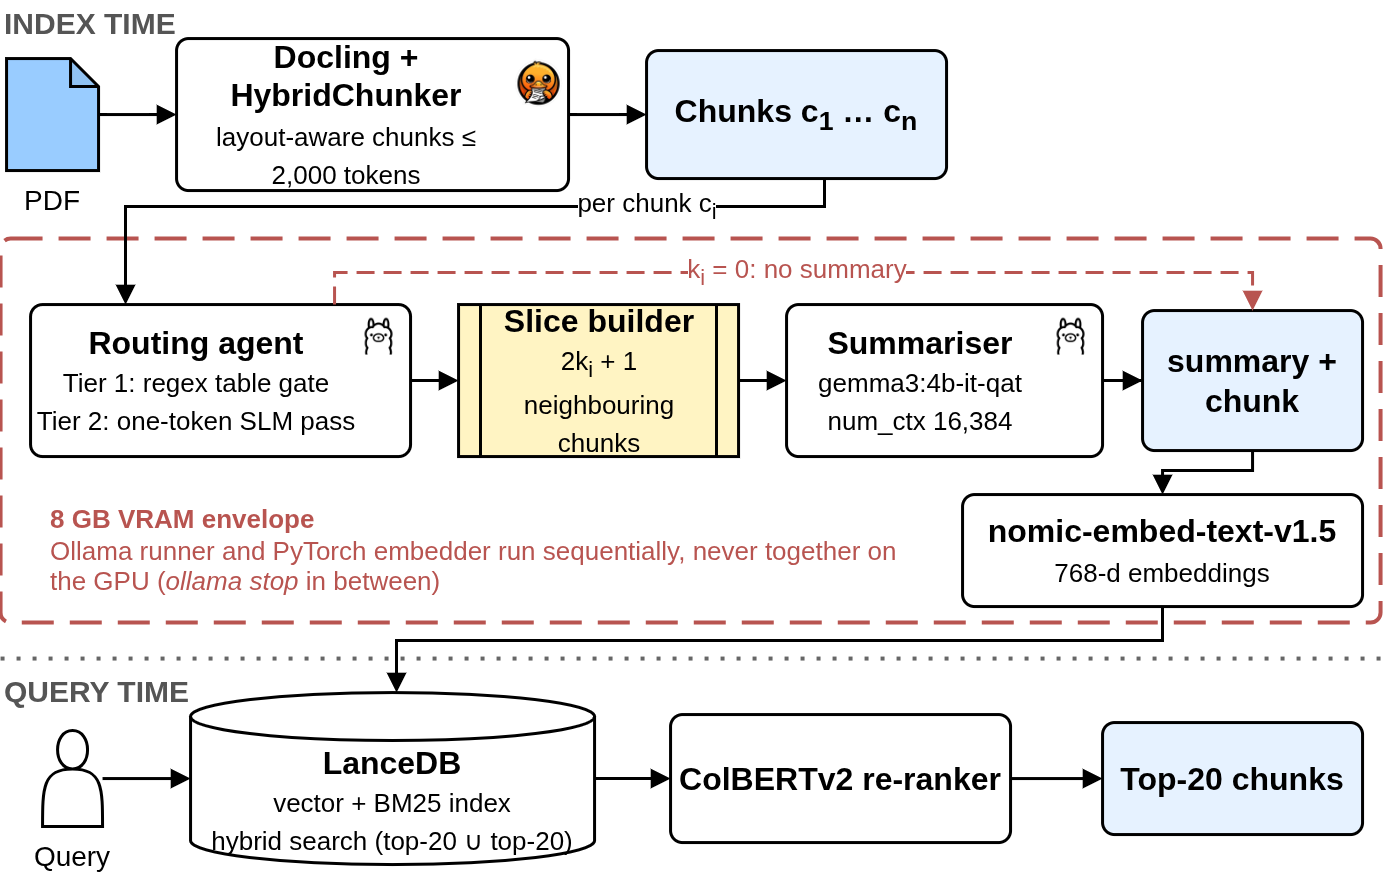
\includegraphics[width=\textwidth]{images/fig01_architecture.png}
  \caption{End-to-end on-premise architecture on one 8\, GB consumer GPU: router and summariser share one resident \texttt{gemma3:4b-it-qat} runner (16\,384-token window), the embedder runs after the runner is stopped, and chunks routed to $k=0$ bypass the summariser.}
  \label{fig:architecture}
\end{figure}

\subsection{Layout-aware document parsing}\label{sec:parsing}

\begin{definition}[Chunk sequence]\label{def:chunks}
Let $\tau$ be the tokenizer of the embedding model and $\ell_{\max}$ a token budget. A document is the ordered chunk sequence
\begin{equation}\label{eq:chunks}
D=(c_1,\dots,c_n),\quad \ell_j=|\tau(c_j)|\le \ell_{\max}=2000,\quad L=\sum_{j=1}^{n}\ell_j,\quad \mathrm{id}(c_j)=\mathrm{SHA256}(\tilde c_j),
\end{equation}
where $\tilde c_j$ is the cleaned chunk text; the content hash gives a chunk the same identifier in every experimental condition.
\end{definition}

Segmentation uses Docling \cite{auer2024doclingtechnicalreport,livathinos2025doclinglayoutanalysis}: layout analysis, table-structure recognition and OCR per page, then the \texttt{HybridChunker} \cite{docling2024chunkingdocumentation} splits along structural elements and merges adjacent elements of a section while the token count under the \texttt{nomic-embed-text-v1.5} tokenizer stays below $\ell_{\max}=2000$, so that a table, its caption and the paragraph discussing it tend to stay together. Chunk text is normalized (Unicode NFKD, ASCII dashes and quotes, URLs removed, whitespace collapsed) before hashing (Fig.~\ref{fig:docling}; Table~\ref{tab:parsing}). Two properties matter later: a recognized table is serialized as one line of ``\texttt{\textless row\textgreater, \textless column\textgreater = \textless value\textgreater.}'' cells, so tables are detectable by a regular expression, and layout artifacts survive (formula placeholders in 51 of the 382 chunks, glyph codes in 93).

\begin{figure}[htbp]
  \centering
  \figbox{3.0cm}{0.94\textwidth}{[FIGURE 2: Docling-based hybrid chunking workflow]}
  \figspec{Boxes: PDF page $\rightarrow$ Docling layout analysis (text blocks, tables, captions, formulas) $\rightarrow$ structural elements $\rightarrow$ HybridChunker (token-bounded merge of peers within a section, nomic tokenizer, 2\,000 tokens) $\rightarrow$ cleaning (NFKD, dash/quote normalisation, URL removal, whitespace) $\rightarrow$ SHA-256 identifier $\rightarrow$ frozen chunk JSON \{text, document, id\}. Annotate a serialized table line (``\texttt{row, column = value.}'') and a formula placeholder as examples of the artifacts the router must cope with.}
  \caption{Layout-aware parsing and chunking: layout analysis, structure-aware segmentation, token-bounded merging of peers within a section, cleaning and hashing.}
  \label{fig:docling}
\end{figure}

\begin{table}[htbp]
\caption{Structural parsing metadata and chunk statistics of the scientific corpus (Docling HybridChunker output).}\label{tab:parsing}
\begin{tabular}{@{}p{5.4cm}p{4.0cm}p{2.8cm}@{}}
\toprule
Quantity & Value & Note \\
\midrule
Documents / chunks & 25 / 382 & 380 distinct identifiers\footnotemark[1] \\
Chunks per document (min/median/max) & 8 / 14 / 33 & token budget 2\,000, merge peers \\
Chunk length, characters (min/median/mean/max) & 4 / 2\,090 / 2\,766 / 10\,260 & total 1\,056\,773 \\
Chunk length, tokens (min/median/mean/max) & 1 / 450 / 666 / 1\,999 & total 253\,488; 4.17 characters per token \\
Chunks per token band ($\le 250$ / 251--500 / 501--1\,000 / 1\,001--1\,500 / 1\,501--2\,000) & 119 / 88 / 78 / 37 / 60 & 25 chunks at $\ge 1\,900$ \\
Document length, tokens (min/median/max) & $\approx$ 4.3k / 10.4k / 18.3k & 17\,760--76\,161 characters \\
Chunks with formula placeholders / glyph codes & 51 / 93 & layout artefacts \\
Chunks carrying a serialised table (Tier-1 gate) & 42 & cells or caption pattern \\
\botrule
\end{tabular}
\footnotetext[1]{The 43-character chunk ``The authors declare no competing interests.'' occurs in three papers and has one identifier; none of the three is a gold chunk.}
\end{table}

\subsection{Bounded document slices}\label{sec:slice}

\begin{definition}[Document slice]\label{def:slice}
For a chunk $c_i\in D$ and a context radius $k\in\mathbb{N}_0$ the document slice is the set of chunks within $k$ positions of $c_i$,
\begin{equation}\label{eq:slice}
\Slice(c_i,k)=\{\,c_j\in D \mid \max(1,\,i-k)\le j\le \min(n,\,i+k)\,\}.
\end{equation}
\end{definition}

Near a document boundary, the implementation compensates the truncated side of Eq.~\eqref{eq:slice} on the other side (Fig.~\ref{fig:clamping}): with $u_i=\max(0,\,k-i+1)$ chunks missing before $c_i$ and $o_i=\max(0,\,i+k-n)$ after it,
\begin{equation}\label{eq:window}
W_i(k)=\bigl\{\,j : \max(1,\,i-k-o_i)\le j\le \min(n,\,i+k+u_i)\,\bigr\},\qquad |W_i(k)|=\min(2k+1,\,n),
\end{equation}
and the target stays central except at the edges, away from the attention-degraded middle of long prompts \cite{liu2023lostmiddlelanguagemodels}. The summariser receives a fixed system prompt (Table~\ref{tab:prompts}), the window text under the header ``\texttt{FULL DOCUMENT:}'' (kept verbatim from the baseline, so that only the content differs between conditions) and the chunk under ``\texttt{CHUNK:}''; its one- or two-sentence answer $s_i$ is prepended to the chunk before embedding. The prompt length of one call is
\begin{equation}\label{eq:prompt}
P_i(k)=s+\sum_{j\in W_i(k)}\ell_j+\ell_i \qquad\text{versus}\qquad P_i^{\mathrm{full}}=s+L+\ell_i
\end{equation}
for the full-document design, with $s=164$ tokens of system prompt, so under $\ell_{\max}=2000$ every slice prompt is bounded by $s+(2k+2)\ell_{\max}$ (12\,190 tokens for $k=2$, 16\,190 for $k=3$) regardless of the document: a fixed 16\,384-token context window suffices for the whole corpus, whereas the full-document baseline needed a 30\,000-token window (Sect.~\ref{sec:complexity}). Note that $k=0$ in the static ablation (Sect.~\ref{sec:static}) still calls the summariser with the chunk as its only context, whereas a radius of $0$ assigned by the router means no summariser call at all.

\begin{figure}[htbp]
  \centering
  \figbox{2.6cm}{0.94\textwidth}{[FIGURE 3: sliding window with boundary clamping, Eq.~\eqref{eq:window}]}
  \figspec{Schematic of Eq.~\eqref{eq:window} for a document of $n=14$ chunks and $k=2$. Three rows of 14 boxes; highlight the window for $i=1$ (chunks 1--5, shifted right by $u_1=2$), $i=7$ (chunks 5--9, centered), and $i=14$ (chunks 10--14, shifted left by $o_{14}=2$); mark the target chunk in each row. The conference figure \texttt{images/underflow\_adjusted\_doc\_slice\_alt.png} (not in the repository) shows the same mechanism and can be reused.}
  \caption{Boundary clamping of the slice window: a side truncated by the document boundary is compensated on the other side, so every prompt carries $\min(2k+1,n)$ chunks and the target stays central except at the edges.}
  \label{fig:clamping}
\end{figure}

\subsection{Dynamic radius routing}\label{sec:router}

Our conference ablation \cite{sandor2025documentslicecontextualretrieval} showed that $k=2$ and $k=3$ are the best fixed radii, but a fixed radius wastes work twice over: chunks that already describe themselves (abstracts, conclusions, reference lists, author and funding statements, layout debris) gain nothing from a summary, and chunks carrying a serialised table are summarised \emph{worse} when the window is wide, because the model then describes the surrounding prose or degenerates into one of its own prompt examples. A routing agent $\mathcal R$ therefore chooses the radius per chunk in two cheap tiers, before any summary is written. Tier~1 is a deterministic table gate,

% Note Formális ellenőrzés eredménye: Táblázat-detektáló kapu (5. egyenlet): A formalizáció itt túlzottan informális és pszeudokód-szerű ("line C c", "#"="(X) \le 100 v caption(c)"). A formális helyesség érdekében ezt szigorúbb halmazelméleti vagy karakterlánc-operátorokra (string matching) épülő szintaktikával kellene definiálni.
\begin{equation}\label{eq:gate}
\mathrm{table}(c)=\Bigl[\exists\,\text{line }\lambda\subseteq c:\ \#\mathrm{cells}(\lambda)\ge 3 \ \wedge\ |\lambda|/\#\text{``\texttt{ = }''}(\lambda)\le 100\Bigr]\ \vee\ \mathrm{caption}(c),
\end{equation}
where a cell matches ``\texttt{, \textless col\textgreater = \textless val\textgreater.}'' and a caption ``\texttt{TABLE I}'', ``\texttt{Table 1:}'' or ``\texttt{Table 1 |}'' at the start of a line; table chunks receive $k_T=2$ without a model call. Tier~2 classifies every other chunk with one forward pass of the resident model emitting a single token, from the router system prompt $\pi_r$ (Table~\ref{tab:prompts}), ten in-context exemplars $\mathcal X$ and the chunk clipped to its first 1\,500 and last 500 characters; the agent takes the argmax of the top-20 next-token log-probabilities over the two answer letters (fallbacks: the emitted token, then $k_{\mathrm{default}}=2$), with $\kappa(\mathrm S)=0$ (self-describing, no summariser call) and $\kappa(\mathrm N)=2$ (needs its neighbours). The policy, and the two statistics reported for every run, are
% Note: Formális ellenőrzés eredménye: Útválasztó ágens döntési függvénye (6. és 7. egyenlet): A darabokra bontott (piecewise) $\mathcal{R}(c_i)$ függvény lefedi az implementációt, de az argmax operátornál a logaritmus valószínűségek kimeneti osztályai hibásan, $\lambda \in \{8, N\}$ formában jelennek meg az elvárt $\{S, N\}$ (Self-describing, Needs neighbours) halmaz helyett. Szintén definiálatlan a 6. egyenlet első ágában szereplő $k_{E,x}$ változó, amely valószínűleg a statikus kísérletek $k$ értékét hivatott jelölni. 
\begin{equation}\label{eq:policy}
\mathcal R(c_i)=
\begin{cases}
k_{\mathrm{fix}} & \text{(control runs)},\\[2pt]
k_T=2 & \text{if } \mathrm{table}(c_i)\ \text{(Tier 1)},\\[2pt]
\kappa\bigl(\arg\max_{\lambda\in\{\mathrm S,\mathrm N\}}\log p_\theta(\lambda\mid \pi_r,\mathcal X,\mathrm{clip}(c_i))\bigr) & \text{(Tier 2)},
\end{cases}
\end{equation}
\begin{equation}\label{eq:kbar}
\bar k=\frac1n\sum_{i=1}^{n}k_i,\qquad N_{\mathrm{calls}}=\bigl|\{\,i : k_i>0\,\}\bigr| .
\end{equation}

One forward pass takes about 0.16\,s on the RTX~4060M (median 155\,ms; the exemplars form a cached prefix of roughly 2\,000 tokens), so the corpus is routed in about a minute, and nothing is reloaded between the routing and summarising phases. With exemplars from six papers outside both benchmarks (109 chunks), the router agrees with a 119-chunk hand-labeled set on 82 of the 99 chunks that reach Tier~2, and the gate fires on all 20 gold table chunks with no false positives. The server's logits vary slightly with the state of its prefix cache, so chunks whose two letters lie within about 0.1--0.3 nats can flip between runs; the agent logs the letter log-probabilities so that such near-ties can be audited, the ``explainable'' half of the pathway of Sect.~\ref{sec:discussion}.

\begin{table}[htbp]
\caption{Prompt templates of the summariser and of the routing agent, and the routing decision criteria.}\label{tab:prompts}
\begin{tabular}{@{}p{2.6cm}p{10.0cm}@{}}
\toprule
Component & Specification \\
\midrule
Summariser & \texttt{gemma3:4b-it-qat} served by Ollama; \texttt{temperature 0}, \texttt{num\_ctx 16384} (\texttt{SYSTEM} block and \texttt{PARAMETER} lines of \texttt{Models/chunker\_full\_doc.Modelfile}, passed per call so that the base model stays resident) \\
Summariser system prompt & 789 characters (164 tokens): return only a short, objective summary of the chunk's relevance, meaning, or contribution to the document as a whole, no preamble, no phrases such as ``This chunk is\ldots''; three one-sentence examples (verbatim in \texttt{Models/chunker\_full\_doc.Modelfile}) \\
Summariser messages & user~1: ``\texttt{FULL DOCUMENT:}'' + newline + the chunks of $W_i(k)$ joined by single spaces; user~2: ``\texttt{CHUNK:}'' + newline + $c_i$; embedded text $s_i$ + blank line + $c_i$ for $k_i>0$, $c_i$ alone for $k_i=0$ (routed) \\
Router & same resident runner and \texttt{num\_ctx}; \texttt{temperature 0}, \texttt{num\_predict 1}, \texttt{top\_p 1}, \texttt{logprobs} with \texttt{top\_logprobs 20}; decision: argmax of the letter log-probabilities, $\kappa(\mathrm S)=0$, $\kappa(\mathrm N)=2$; fallback: parse the emitted letter, else $k_{\mathrm{default}}=2$ \\
Router system prompt & ``Decide whether the passage describes itself'': S\,--\,self-describing (abstract; conclusion or summary of the whole paper, even when full of numbers; non-content matter such as reference lists, acknowledgements, funding, author biographies, competing interests, metadata, licence text, layout garbage); N\,--\, needs its neighbours (any other passage); ``Reply with the letter only'' (verbatim: \texttt{BINARY\_SYSTEM\_PROMPT} in the repository) \\
Router user message & ten exemplar blocks ``\texttt{Passage:} $x$ / \texttt{Answer:} S$\mid$N'' (from six held-out papers: abstract, reference-list excerpt, conclusion, acknowledgement $\to$ S; formula block, related work, caption fragment, results, device description, experimental setup $\to$ N), then ``\texttt{Passage:} $\mathrm{clip}(c_i)$ / \texttt{Answer:}'' with the query clipped to its first 1\,500 and last 500 characters \\
Tier-1 criteria & $\ge 3$ cells ``\texttt{, \textless col\textgreater = \textless val\textgreater.}'' on one line with $\le 100$ characters per ``\texttt{ = }'', or a caption ``\texttt{TABLE I}'' / ``\texttt{Table 1:}'' / ``\texttt{Table 1 |}'' at the start of a line $\Rightarrow k_T=2$ \\
\botrule
\end{tabular}
\end{table}

\subsection{Context-enriched embedding and hybrid retrieval}\label{sec:retrieval}

The enriched text is embedded with \texttt{nomic-embed-text-v1.5} \cite{nussbaum2024nomic}, a 768-dimensional open-weight encoder with a long native context and a competitive MTEB score \cite{muennighoff2023mteb} that runs unquantized on the same GPU, through LanceDB's embedding registry \cite{lancedb} in fp32 with mean pooling, without task prefixes or normalization, identically in every condition. LanceDB stores the enriched text with its vector, a BM25 index, the raw chunk, the summary, the content hash, and the routing decision. Retrieval is hybrid \cite{kiran2025hybrid,wang2024searching}: the 20 nearest chunks by exact L2 search and the 20 best BM25 matches \cite{robertson1995okapi,robertson2009bm25} are re-scored by a ColBERTv2 re-ranker \cite{khattab2020colbert,santhanam2022colbertv2} and cut to the top 20. Every system, including the full-document baseline and the no-context control, is indexed and queried with exactly this procedure, so the only experimental variable is the embedded text. The Ollama runner and the PyTorch models cannot share the GPU without spilling, so the phases run in sequence (routing and summarisation, \texttt{ollama stop}, embedding and indexing, retrieval); Table~\ref{tab:hardware} lists the environment.

\begin{table}[htbp]
\caption{Experimental hardware and software environment and embedding configuration.}\label{tab:hardware}
\begin{tabular}{@{}p{3.2cm}p{9.4cm}@{}}
\toprule
Item & Specification \\
\midrule
CPU / system memory & Intel Core i7-14650HX, 24 threads / 31.06\,GB \\
GPU & NVIDIA GeForce RTX 4060 Laptop GPU, 8\,GB VRAM; memory bandwidth 256 GB/s; peak use 7\,695\,MiB over the full pipeline; resident summariser runner 4.54\,GiB (16\,384-token window) and 4.82\,GiB (30\,000), all layers on the device (Sect.~\ref{sec:profiling}) \\
OS / Python/server & Linux (zen kernels 6.18--7.2); Python 3.13 (spring and summer 2026 runs) and 3.12 (router study); Ollama 0.17.5 (March 2026 runs), 0.32.1 (July policy-corpus runs), 0.34.0 and 0.34.3 (September router runs), 0.35.1 (memory measurements); one resident runner \\
Summariser and router model & \texttt{gemma3:4b-it-qat} (Gemma~3, 4B parameters, quantisation-aware trained int4 weights \cite{gemma3report2025,jacob2018quantization}); 34 layers, $n_g=5$ global and $n_s=29$ sliding-window (1\,024 tokens), $n_{kv}=4$ key--value heads of width $d_h=256$, fp16 cache ($b=2$) \\
Context window (\texttt{num\_ctx}) & 16\,384 tokens for the slice and routed pipelines (KV cache 494\,MiB); 30\,000 tokens for the full-document baseline (764\,MiB) \\
Embedding model & \texttt{nomic-ai/nomic-embed-text-v1.5}, 768-d, mean pooling, fp32 on CUDA via the LanceDB HuggingFace registry \\
Vector store / search & LanceDB 0.26.1; hybrid = exact-L2 vector top-20 $\cup$ BM25 top-20 $\rightarrow$ ColBERTv2 (\texttt{colbert-ir/colbertv2.0}) re-rank $\rightarrow$ 20 \\
Parsing / chunking & docling 2.68.0, docling-core 2.59.0 (HybridChunker, RapidOCR); transformers 4.57.5; torch 2.9.1 \\
Energy tracking & CodeCarbon 3.2.3 (spring/summer 2026 rows) and 3.3.1 (September 2026 rows) \\
\botrule
\end{tabular}
\ifprovenance\footnotetext{\verify{CPU, GPU, RAM, OS, Python and CodeCarbon versions: columns \texttt{cpu\_model}, \texttt{gpu\_model}, \texttt{ram\_total\_size}, \texttt{os}, \texttt{python\_version}, \texttt{codecarbon\_version} of \texttt{RnD/emissions\_data/emissions.csv} (rows written by CodeCarbon 3.3.1 are shifted by two columns from \texttt{region} onward relative to the 3.2.3 header; read those rows by position). Library versions: \texttt{RnD/requirements.txt}. Context windows: the two Modelfiles in \texttt{RnD/Models/}. Peak memory: \texttt{README.md} line~59. Runner footprint and cache sizes: \texttt{RnD/verification/ollama\_runner\_vram.json} and the \texttt{llama\_kv\_cache} log lines in \texttt{ollama\_offload\_pressure\_v0.35.1\_ballast0.json}; model constants from the same server log (5 global and 29 SWA layers, \texttt{n\_embd\_head\_k} 256, 4 KV heads) and the Gemma~3 report. Server versions: \texttt{/var/log/pacman.log} (ollama 0.17.5 from 2026-03-02, 0.32.1 from 2026-07-18, 0.34.0 from 2026-09-11, 0.34.3 from 2026-09-24, 0.35.1 from 2026-10-03).}}\fi
\end{table}

\subsection{Computational complexity and memory analysis}\label{sec:complexity}

Index-time contextualization issues one summariser call per chunk, so a document costs the sum of Eq.~\eqref{eq:prompt}. With $\bar\ell=L/n$ and the system prompt neglected, the prompt-token volumes of the three designs are
\begin{align}
C_{\mathrm{full}}&=\sum_{i=1}^{n}(L+\ell_i)=(n+1)L,\qquad
C_{k}=\sum_{i=1}^{n}\Bigl(\sum_{j\in W_i(k)}\ell_j+\ell_i\Bigr)\le n\,(2k+2)\,\ell_{\max},\nonumber\\
C_{\mathrm{dyn}}&=\sum_{i:\,k_i>0}\Bigl(\sum_{j\in W_i(k_i)}\ell_j+\ell_i\Bigr)+\sum_{i\notin\mathcal T}\rho_i,\label{eq:volume}
\end{align}
where $\mathcal T$ is the set of table-gated chunks and $\rho_i$ the router prompt (about 2\,000 tokens, mostly a cached prefix)\verify{router prompt length: mean 2\,062 tokens printed by \texttt{RnD/ollama\_dynamic\_slice\_length.ipynb}}: the full-document volume is quadratic in $n$, the bounded volume linear with a constant $2k+2$ that the router lowers further by skipping chunks. Attention widens the gap, since a forward pass over $P$ tokens costs approximately \cite{kaplan2020scaling}
\begin{equation}\label{eq:flops}
F(P)\approx 2N_{\mathrm{par}}\,P+2\,n_L\,d_{\mathrm{attn}}\,P^{2}
\end{equation}
($N_{\mathrm{par}}$ non-embedding parameters, $n_L$ layers, attention width $d_{\mathrm{attn}}$), so a document's attention work is $\propto\sum_i P_i^2$.

\begin{proposition}[Asymptotic index-time cost]\label{prop:complexity}
Let every chunk satisfy $\ell_j\le\ell_{\max}$ and let $n\ge 2k+1$. Then the attention work of full-document contextualisation grows as $\sum_i (L+\ell_i)^2=\Theta(n^{3}\bar\ell^{\,2})$, while that of Document Slice contextualisation with radius $k$ is bounded by $\sum_i P_i(k)^2\le n\,(2k+2)^2\ell_{\max}^2=\Theta(n\,\ell_{\max}^2)$; the designs differ by $\Theta\bigl(n^2/(2k+2)^2\bigr)$ in attention work and $\Theta\bigl(n/(2k+2)\bigr)$ in prompt tokens.
\end{proposition}
\begin{proof}
$L\le L+\ell_i\le 2L$ with $L=n\bar\ell$ gives $n^3\bar\ell^{\,2}\le\sum_i(L+\ell_i)^2\le 4n^3\bar\ell^{\,2}$; by Eq.~\eqref{eq:window} the window holds $2k+1$ chunks, so $P_i(k)\le(2k+2)\ell_{\max}$, and $\sum_i P_i(k)^2\ge n\bar\ell^{\,2}$ by Cauchy--Schwarz, the two being of the same order for token-bounded chunkers. The token statement follows from Eq.~\eqref{eq:volume}.
\end{proof}

On the corpus the bounds are loose but the ordering holds (Fig.~\ref{fig:complexity}): the full-document design sends 18.73\,M characters ($\approx 4.5$\,M tokens) to the summariser, fixed $k=1,\dots,4$ send 4.25, 6.36, 8.43 and 10.32\,M, and the routed pipeline 4.39\,M (23.4\,\% of the baseline) in 261 instead of 382 calls; $\sum_i P_i^2$ is 4.6 times smaller for $k=3$ and 10.8 times smaller for the routed pipeline than for the baseline, and the measured generation-time ratio of 6.3 (Sect.~\ref{sec:primary}) lies between this quadratic proxy and the linear one (4.3).\verify{re-implementation of the \texttt{cost()} formula of \texttt{RnD/dynamic\_slice\_length/router\_experiments/scripts/cost.py} (window characters of Eq.~\eqref{eq:window} plus the chunk, summed over \texttt{RnD/split\_documents/*.json}; the full-document prompt is the space-joined document plus the chunk; the routed radii are the \texttt{doc\_slice\_radius} fields of \texttt{RnD/preprocessed\_chunks/ablation\_doc\_slice\_radius\_dynamic.json}): 18\,728\,428 / 4\,254\,674 / 6\,360\,511 / 8\,433\,157 / 10\,320\,971 / 4\,391\,194 characters; $\sum P_i^2$ ratios 4.56 and 10.81; tokens $\approx$ characters$/4.17$; the mean $k=2$ prompt is $6\,360\,511/382/4.17+190\approx 4\,180$ tokens against the 12\,190-token bound; script \texttt{RnD/verification/prompt\_volume\_and\_attention\_proxy.py}}

\begin{figure}[htbp]
  \centering
  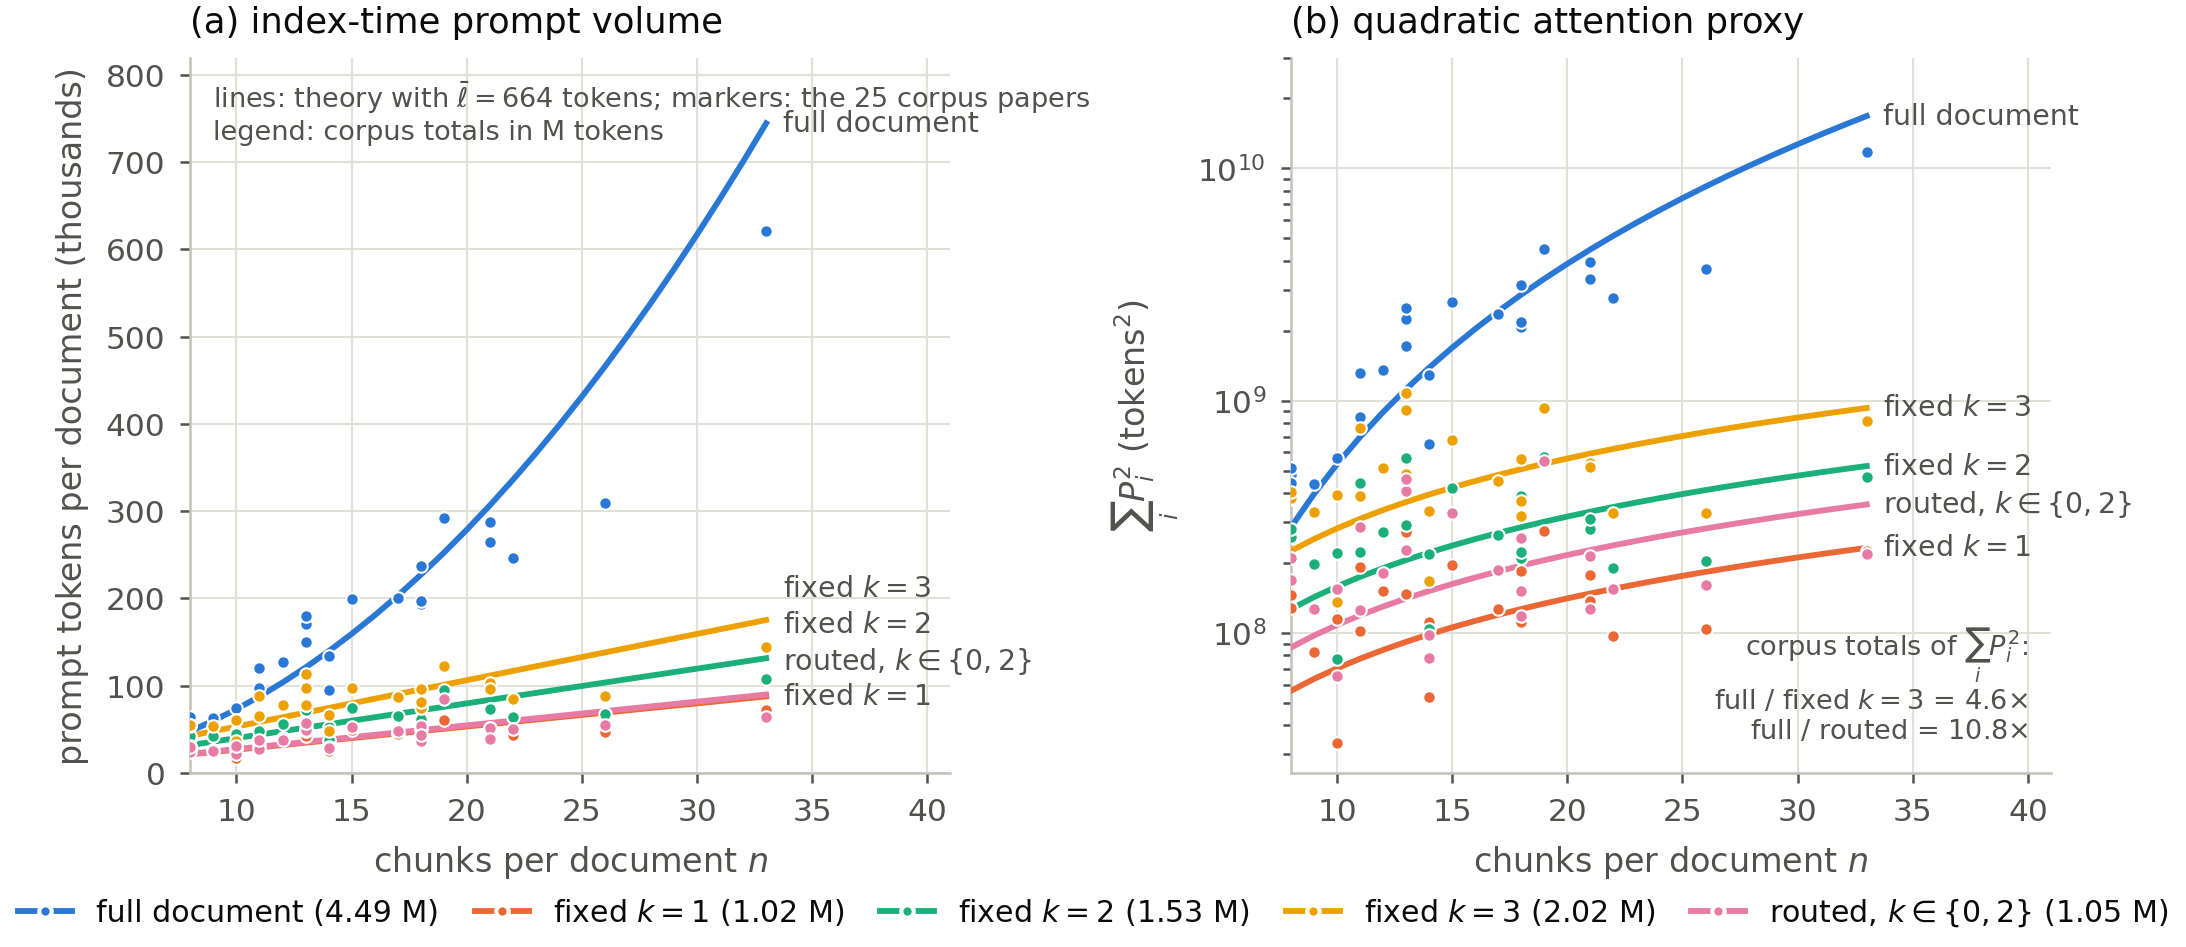
\includegraphics[width=\textwidth]{images/fig04_cost_curves.png}
  \label{fig:complexity}
\end{figure}

Memory decides whether the arithmetic can be done on the device at all: the GPU must hold the quantized weights $M_w$, the activations $M_{\mathrm{act}}$, and the KV cache, which for $P$ tokens occupies
\begin{equation}\label{eq:kv}
M_{\mathrm{KV}}(P)=2\,n_L\,n_{kv}\,d_h\,b\,P
\end{equation}
bytes ($n_{kv}$ key--value heads of width $d_h$, $b$ bytes per element) \cite{pope2023efficiently,ainslie2023gqa}, so the run stays on the device only if
\begin{equation}\label{eq:vram}
M_w+M_{\mathrm{KV}}(P_{\mathrm{ctx}})+M_{\mathrm{act}}\le V_{\mathrm{GPU}}
\quad\Longleftrightarrow\quad
P_{\mathrm{ctx}}\le P^{\star}=\frac{V_{\mathrm{GPU}}-M_w-M_{\mathrm{act}}}{2\,n_L\,n_{kv}\,d_h\,b},
\end{equation}
where $P_{\mathrm{ctx}}$ is the window reserved at load time, not the current prompt length. The bounded slice fixes $P_{\mathrm{ctx}}=16\,384$ for every document ($k\le3$); the full-document design needs $P_{\mathrm{ctx}}\ge s+L_{\max}+\ell_{\max}$, about 18\,300 tokens for the longest paper, and was run with a 30\,000-token window\verify{longest document 76\,161 characters (sum of chunk lengths of \texttt{s41586-019-1138-y.pdf.json} in \texttt{RnD/split\_documents/}), divided by 4.17 characters per token; windows from \texttt{RnD/Models/chunker\_anthropic.Modelfile} (30000) and \texttt{chunker\_full\_doc.Modelfile} (16384)}. What the wider window costs depends on the cache architecture. For a dense cache, Eq.~\eqref{eq:kv} with the constants of an 8B model of 32 layers and 8 key--value heads of width 128 gives 3.7\,GiB at 30\,000 and 2.0\,GiB at 16\,384 tokens in fp16, so next to about 4.6\,GiB of int4 weights the wider window no longer fits an 8\,GiB device while the bounded one does. Gemma~3 interleaves $n_s=29$ local layers, whose cache is capped at the sliding window of 1\,024 tokens, with $n_g=5$ global layers, so only the global share grows with the window:
\begin{equation}\label{eq:kv-iswa}
M_{\mathrm{KV}}(P_{\mathrm{ctx}})=2\,n_{kv}\,d_h\,b\,\bigl(n_g\,P_{\mathrm{ctx}}+n_s\,\tilde w\bigr),
\end{equation}
with $\tilde w=1\,536$ cells (window plus batch). The server allocates 764\,MiB at 30\,000 and 494\,MiB at 16\,384 tokens, and the resident runner measures 4.82 against 4.54\,GiB on an otherwise empty device, every layer on the GPU in both cases, under the server release of the March runs as well as the current one.\verify{cache: \texttt{llama\_kv\_cache} lines (590 + 174 and 320 + 174\,MiB) in the \texttt{log} field of \texttt{RnD/verification/ollama\_offload\_pressure\_v0.35.1\_ballast0.json} and the \texttt{required.CUDA0.Cache} vector ($5\times123\,731\,968 + 29\times6\,291\,456$ bytes) in \texttt{\ldots\_v0.17.5\_ballast0.json}; Eq.~\eqref{eq:kv-iswa} with $n_{kv}=4$, $d_h=256$, $b=2$, 30\,208 cells reproduces 764\,MiB; footprint: (\texttt{peak\_mib} $-$ \texttt{idle\_mib})/1024 of \texttt{RnD/verification/ollama\_runner\_vram.json} (4\,947 and 4\,663\,MiB, Ollama 0.35.1; 4\,995 and 4\,711\,MiB with 0.17.5 in \texttt{ollama\_offload\_pressure\_v0.17.5\_ballast0.json}); ``offloaded 35/35 layers'' in both logs; scripts \texttt{ollama\_runner\_vram.py}, \texttt{ollama\_offload\_under\_vram\_pressure.py}} For this model the reserved window therefore does not cross $P^{\star}$ on an 8\,GiB device by itself; what crosses it is the memory that other components of the pipeline hold at the same time, which Sect.~\ref{sec:profiling} measures.

\subsection{Evaluation metrics and statistical protocol}\label{sec:metrics}

For a question $q\in Q$ let $G_q$ be its gold chunks, $R_q^K$ the top-$K$ retrieved list and $\rnk_q(c)$ the 1-based position of $c$ in it; for $K\in\{5,10,15,20\}$ we report
\begin{align}
\Rec{K}&=\frac{1}{|Q|}\sum_{q\in Q}\frac{|R_q^K\cap G_q|}{|G_q|},\qquad
Q_K^{+}=\{\,q\in Q : R_q^K\cap G_q\neq\varnothing\,\},\label{eq:recall}\\
\MRR{K}&=\frac{1}{|Q_K^{+}|}\sum_{q\in Q_K^{+}}\frac{1}{\min_{c\in R_q^K\cap G_q}\rnk_q(c)},\label{eq:mrr}\\
\MAR{K}&=\frac{1}{|Q_K^{+}|}\sum_{q\in Q_K^{+}}\frac{1}{|R_q^K\cap G_q|}\sum_{c\in R_q^K\cap G_q}\rnk_q(c).\label{eq:mar}
\end{align}
Recall is primary because every question needs at least two chunks; MRR \cite{voorhees1999trec8} reflects the first relevant chunk; MAR, our exploratory measure of attentional accessibility, is the mean position of \emph{all} retrieved gold chunks and tells whether the evidence sits where the positional bias of Sect.~\ref{sec:intro} is least harmful. Ranking metrics are averaged over $Q_K^{+}$ (questions without a hit are excluded rather than scored zero; 233, 246, 247 and 248 of 250 for the routed pipeline)\verify{``Number of N values with NaN MRR in own metrics: 17/250, 4/250, 3/250, 2/250'' printed by cell~7 of \texttt{RnD/benchmarking\_retrievals.ipynb}; the \texttt{np.nanmean} calls in cell~9 implement the exclusion}, and gold sets are matched by content hash. \Rec{20} differences are tested per question with a 99\,\% BCa bootstrap interval of the paired difference \cite{efron1987better,smucker2007comparison} (SciPy \cite{virtanen2020scipy}, 9\,999 resamples, fixed seed) and an exact McNemar test \cite{McNemar_1947,dietterich1998approximate} on the event ``all gold chunks in the top 20'', reporting the discordant counts $b$ (only the compared system succeeds) and $c$ (only the baseline succeeds). Because the summariser is stochastic even at temperature~0, we also measure the noise floor of a single run by regenerating one configuration (Sect.~\ref{sec:routing-results}): about 0.7 points of \Rec{20} and 2 points of \MRR{20}, below which gaps are treated as ties.

% Note: Ezt én inkább az elején letudnám a módszertanban. Általában ott szokott lenni ha csak nincs valamilyen különleges oka hogy végén mutassuk be.
\subsection{Datasets}\label{sec:datasets}

The primary corpus consists of 25 open-access papers from IEEE and Nature-portfolio journals across engineering, physics, computing, and the life sciences, chosen for their heavy use of tables, formulas, and figure references. Following the LLM-as-a-judge paradigm \cite{zheng2023judgingllmasajudgemtbenchchatbot} we built a ``silver standard'' question set \cite{rebholz2010silverstandard}: Gemini~3~Pro was given the chunk JSON of one paper at a time and instructed to write exactly ten high-complexity question--answer pairs grounded only in the provided text, each requiring at least two distinct chunk identifiers (abridged prompt in the conference paper \cite{sandor2025documentslicecontextualretrieval}), and a validator rejects questions with fewer than two supporting chunks or with unknown identifiers: 250 questions with 530 gold references over 226 distinct chunks (Table~\ref{tab:corpora}). The gold labels come from a large proprietary model and the summaries from a 4-billion-parameter open model, so a shared preference for particular chunks is unlikely. To test the method inside the target genre of regulatory text, we use four public European Commission documents on tobacco-control policy (COM(2016)~269, COM(2021)~249, SWD(2013)~56 and the 2023 methodology report of the Independent Advisory Panel on characterising flavours), chunked and questioned with the same protocol (80 questions, 164 gold references; a random 20\,\% subset was checked manually); they share the genre of energy-governance documents: directive articles, member-state implementation tables, methodology sections and annexes. The router's exemplars come from six further papers in neither benchmark, so no text the router has seen as an example can be retrieved as an answer.\verify{\texttt{RnD/split\_documents\_router/}: 6 files, 109 records; \texttt{RnD/input\_router/} holds the PDFs}

\begin{table}[htbp]
\caption{Evaluation corpora: the scientific silver-standard benchmark and the European Commission policy set.}\label{tab:corpora}
\begin{tabular}{@{}p{4.0cm}p{4.0cm}p{4.2cm}@{}}
\toprule
Quantity & Scientific benchmark & EC policy set \\
\midrule
Documents & 25 (IEEE, Nature portfolio) & 4 (COM(2016)~269, COM(2021)~249, SWD(2013)~56, IAP methodology 2023) \\
Chunks & 382 & 141 (14 / 32 / 35 / 60 per document) \\
Characters (total) / median chunk length & 1\,056\,773 / 2\,090 & 259\,985 / 1\,206 \\
Chunk length, tokens (mean / median) & 663.6 / 450 & 446.8 / 246 \\
Questions & 250 (10 per document) & 80 (10 / 20 / 20 / 30 per document) \\
Supporting chunks per question & 2--4 (mean 2.12; 223 / 24 / 3 questions with 2 / 3 / 4) & 2--3 (mean 2.05; 76 / 4) \\
Gold references & 530 & 164 \\
Distinct gold chunks (share of corpus) & 226 (59.5\,\%) & 94 (66.7\,\%) \\
Question generator / manual validation & Gemini~3~Pro / --- & Gemini~3~Pro / 20\,\% random subset \\
\botrule
\end{tabular}
\ifprovenance\footnotetext{\verify{Chunk counts, character statistics and per-document chunk counts: read-only pass over \texttt{RnD/split\_documents/*.json} and \texttt{RnD/split\_documents/smoking/*.json}; question statistics: \texttt{RnD/q\_and\_a/Gemini/scientific\_multi\_chunk\_control.json} and \texttt{RnD/q\_and\_a/Gemini/smoking.json} (count the \texttt{supporting\_chunks} lists; distinct gold ids as a set); token statistics: \texttt{len(tokenizer.tokenize(text))} with the nomic tokenizer over \texttt{RnD/split\_documents/*.json} (mean 663.58, median 450, total 253\,488) and over the final 141 records of \texttt{RnD/split\_documents/smoking/*.json} (mean 446.80, median 246, min 1, max 1\,992, total 62\,999); the 420.94 printed by cell~2 of \texttt{RnD/doc\_slice\_chunking.ipynb} refers to an earlier 144-chunk version of the policy corpus; scripts: \texttt{RnD/verification/chunk\_character\_statistics.py} and \texttt{chunk\_token\_statistics.py}.}}\fi
\end{table}

\subsection{Continuous energy and carbon accounting}\label{sec:energy}

Every generation run is wrapped in a CodeCarbon tracker \cite{codecarbon_software,lacoste2019quantifyingcarbonemissionsmachine} that samples GPU, CPU, and memory power once per second and integrates it over the run; emissions follow through the grid factor:
\begin{equation}\label{eq:energy}
E_{\mathrm{total}}=\int_{0}^{T}\bigl(P_{\mathrm{GPU}}(t)+P_{\mathrm{CPU}}(t)+P_{\mathrm{DRAM}}(t)\bigr)\,dt
\;\approx\;\sum_{t=1}^{\lceil T/\Delta t\rceil}\bigl(P^{(t)}_{\mathrm{GPU}}+P^{(t)}_{\mathrm{CPU}}+P^{(t)}_{\mathrm{DRAM}}\bigr)\,\Delta t,
\end{equation}
\begin{equation}\label{eq:emissions}
\mathrm{Emissions}=E_{\mathrm{total}}\times\mathrm{CI}_{\mathrm{grid}}\times\mathrm{PUE},
\end{equation}
with $\Delta t=1$\,s, where $\mathrm{CI}_{\mathrm{grid}}$ is the operational carbon intensity of the regional grid in \gco{} per kWh and the power-usage effectiveness is 1 for a workstation. GPU power is read from NVML; CPU power came from RAPL counters for the spring-2026 runs and from a load-based estimate for the later runs; memory power is a constant estimate (Table~\ref{tab:power}). Energy is therefore the primary efficiency metric, and GPU energy, measured consistently throughout, is reported alongside the total as the component comparable without qualification.\verify{measurement methods: the CodeCarbon start-up messages saved in \texttt{RnD/anthropic\_traditional\_chunking.ipynb} (March: ``Tracking Intel CPU via RAPL interface''; July: ``RAPL -- Permission denied \ldots Falling back on CPU load mode''); the grid factor is \texttt{emissions}/\texttt{energy\_consumed} of each row of \texttt{RnD/emissions\_data/emissions.csv} (204.19 for the four 3.2.3 rows; 211.50--214.03 for the complete 3.3.1 rows)} Durations come in two scopes: the \emph{tracked generation scope}, the interval wrapped by the tracker (routing and summarisation over pre-chunked documents, without PDF parsing, embedding or indexing), to which all energy figures refer; and the \emph{end-to-end preprocessing scope}, including PDF conversion, to which the conference paper's headline times (71\,min~34\,s baseline, 29\,min~09\,s fixed $k=3$) belong.

\begin{table}[htbp]
\caption{Power-measurement coefficients, per-run power draw, and grid emission factors.}\label{tab:power}
\begin{tabular}{@{}p{5.5cm}p{7.1cm}@{}}
\toprule
Quantity & Value \\
\midrule
Sampling interval / tracking mode / PUE & 1\,s / whole machine / 1.0 \\
GPU power & measured via NVML (all runs) \\
CPU power & RAPL counters (runs of 5 March 2026); load-based estimate with the tracker's TDP fallback (``4\,W per thread $\times$ 24 threads $=$ 96\,W'') from 19 July 2026 on \\
Memory power & constant 20.0\,W estimate (31\,GB installed) \\
Grid carbon intensity (Hungary) & 204.19\,\gco{}/kWh (CodeCarbon 3.2.3 data set); effective 211.5--214.0\,\gco{}/kWh in the 3.3.1 rows \\
Mean GPU power / utilisation: baseline; static $k=3$; routed & 51.5\,W / 46.5\,\%; 55.0\,W / 60.6\,\%; 62.5\,W / 90.1\,\% \\
Mean CPU power: baseline; $k=3$ (RAPL); routed (estimate) & 46.1\,W; 58.0\,W; 10.4\,W \\
Mean host memory in use: baseline / $k=3$ / routed & 15.9 / 19.4 / 17.3\,GB \\
Water footprint & not tracked (WUE 0) \\
\botrule
\end{tabular}
\ifprovenance\footnotetext{\verify{All rows are columns of \texttt{RnD/emissions\_data/emissions.csv}: \texttt{gpu\_power}, \texttt{gpu\_utilization\_percent}, \texttt{cpu\_power}, \texttt{ram\_used\_gb}, \texttt{ram\_power}, \texttt{pue}, \texttt{tracking\_mode} of the rows timestamped 2026-03-05T23:59:43 (baseline), 2026-03-05T22:53:27 (static $k=3$) and 2026-09-25T20:06:47 (routed); the TDP fallback message is in the saved CodeCarbon log of \texttt{RnD/anthropic\_traditional\_chunking.ipynb}. Rows written by CodeCarbon 3.3.1 must be read by position (two-column shift after \texttt{region}).}}\fi
\end{table}

\section{Results and empirical evaluation}\label{sec:results}

% Note: Mivel vannak alszekciók itt is egy kicsit kontextusba helyezheted mi következik az alszekciókban ugyanúgy ahogy a methodolgy-ban is csináltad.
All metrics are those of Sect.~\ref{sec:metrics} on the corpora of Sect.~\ref{sec:datasets}; times and energies refer to the tracked generation scope unless stated otherwise.

\subsection{Static radius sweep}\label{sec:static}

Table~\ref{tab:sweep} and Fig.~\ref{fig:heatmap} report the fixed-radius ablation that motivated the router. Generation time grows linearly with the radius, about five minutes per unit of $k$ over the 382 chunks, while recall saturates: $k=2$ and $k=3$ are the best fixed radii (\Rec{20} of 0.94667 and 0.94533) and $k=4$ falls back to the level of $k=1$ (0.94333) although it sends 62\,\% more prompt text than $k=2$.\verify{times: the ``k=0 \ldots k=4'' comment block in cell~1 of \texttt{RnD/ablation\_doc\_slice\_generation.ipynb} (wall-clock of the generation loop, no tracker); recall values: ``METRICS AT N=20'' blocks of \texttt{RnD/ablation\_doc\_slice\_retrieval.ipynb} for the tables \texttt{ablation\_doc\_slice\_radius\_0..4}; prompt-text ratio $10\,320\,971/6\,360\,511=1.62$ from the \texttt{cost.py} re-implementation} The full-document baseline remains the most accurate (0.95400) at 54\,min~54\,s and 106.7\, Wh, and even the no-context control reaches 0.93933, so contextualisation is worth about 1.5 points on this benchmark, most of it from the immediate neighbourhood of a chunk. All recall differences among $k\in\{1,\dots,4\}$ lie inside the single-run noise band (Sect.~\ref{sec:routing-results}): the sweep identifies a plateau, not an optimum, which is where a per-chunk decision can save cost without losing accuracy.

\begin{table}[htbp]
\caption{Ablation over static window radii versus full-document context and the routed pipeline (250 questions).}\label{tab:sweep}
\setlength{\tabcolsep}{4pt}
\begin{tabular}{@{}p{3.7cm}ccccc@{}}
\toprule
Method & Time (min:s) & Prompt (M chars) & \Rec{20} & \MRR{20} & \MAR{20} \\
\midrule
No context (hybrid only) & --- & 0 & 0.93933 & 0.77484 & 4.03629 \\
Slice $k=0$ (chunk-only summary) & 7:28\footnotemark[1] & 2.11 & 0.93733 & 0.78612 & 3.80827 \\
Slice $k=1$ & 12:08\footnotemark[1] & 4.25 & 0.94333 & 0.79900 & 3.72605 \\
Slice $k=2$ & 17:28\footnotemark[1] & 6.36 & 0.94667 & 0.76799 & 3.80948 \\
Slice $k=3$ & 22:41\footnotemark[1] & 8.43 & 0.94533 & 0.78774 & 4.01999 \\
Slice $k=4$ & 28:11\footnotemark[1] & 10.32 & 0.94333 & 0.78335\footnotemark[2] & 3.95884 \\
Full document (baseline) & 54:54 & 18.73 & 0.95400 & 0.78635 & 3.93548 \\
Routed (this work) & 8:45 & 4.39 & 0.95200 & 0.79798 & 3.91062 \\
\botrule
\end{tabular}
\footnotetext[1]{Wall-clock of the generation loop as recorded in the notebook; these runs were not energy-tracked. Energies of the baseline, the static $k=3$ slice and the routed pipeline are in Table~\ref{tab:primary}.}
\footnotetext[2]{The conference paper printed 0.8933; 0.78335 is the value in the evaluation notebook.}
\ifprovenance\footnotetext{\verify{Recall/MRR/MAR: ``METRICS AT N=20'' printouts in \texttt{RnD/ablation\_doc\_slice\_retrieval.ipynb} (tables \texttt{hybrid\_retrieval}, \texttt{ablation\_doc\_slice\_radius\_0..4}, \texttt{anthropic\_control\_table}) and in \texttt{RnD/benchmarking\_retrievals.ipynb} (routed row, own vs baseline). Times: cell~1 comments of \texttt{RnD/ablation\_doc\_slice\_generation.ipynb} for $k=0..4$; \texttt{duration} column of \texttt{RnD/emissions\_data/emissions.csv} for the baseline (3\,294.3\,s, row 2026-03-05T23:59:43) and the routed run (525.3\,s, row 2026-09-25T20:06:47). Energy: \texttt{energy\_consumed} of the same rows and of row 2026-03-05T22:53:27 ($k=3$). Prompt volumes: \texttt{cost.py} re-implementation (Sect.~\ref{sec:complexity}).}}\fi
\end{table}

\begin{figure}[htbp]
  \centering
  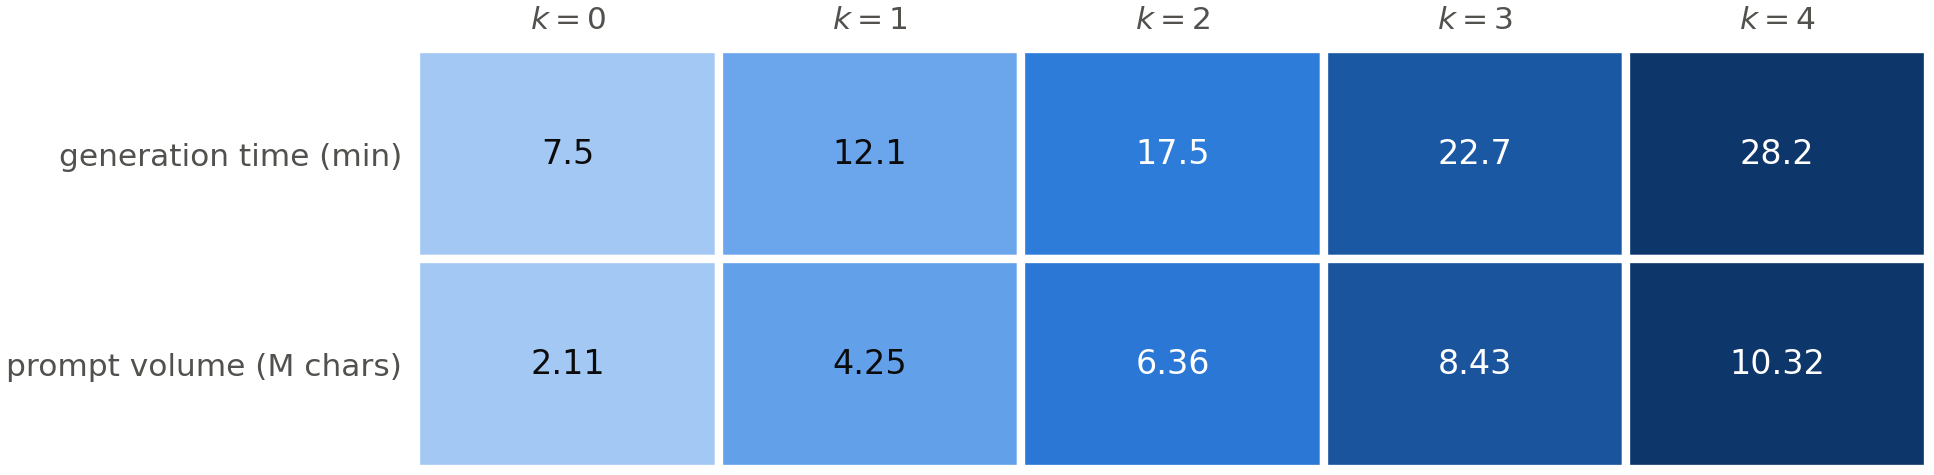
\includegraphics[width=\textwidth]{images/fig06_radius_heatmap.png}
  \caption{Cost surface of the static radius: generation time grows linearly in $k$ and prompt volume with $2k+2$ (notebook wall-clock of the generation loop over 382 chunks; $k=0$ still calls the summariser with the chunk alone), while the reserved context window, and with it the resident device memory of the runner, stays at 4.54\,GiB for every $k$ (Sect.~\ref{sec:profiling}).}
  \verify{times: cell~1 comments of \texttt{RnD/ablation\_doc\_slice\_generation.ipynb} (7m28s, 12m08s, 17m28s, 22m41s, 28m11s); volumes: \texttt{RnD/verification/prompt\_volume\_and\_attention\_proxy.py}; 4.54\,GiB: \texttt{RnD/verification/ollama\_runner\_vram.json}; drawn by \texttt{RnD/citds\_article/figures/fig06\_radius\_heatmap.py}}
  \label{fig:heatmap}
\end{figure}

\subsection{Primary benchmark: full-document baseline, static slice and routed pipeline}\label{sec:primary}

Table~\ref{tab:primary} is the central result. The routed pipeline reaches \Rec{20} of 0.952 against 0.954 for the full-document baseline and 0.94533 for the static $k=3$ slice, both differences inside the single-run band, with the best \MRR{20}, \MAR{20} and \Rec{5} of the three; the recall trajectories (Fig.~\ref{fig:recall}) show it ahead at $K=5$ and $10$, 0.7 points behind at $K=15$ and 0.2 at $K=20$.\verify{routed and baseline values: the four ``METRICS AT N='' blocks of \texttt{RnD/benchmarking\_retrievals.ipynb} (OWN = \texttt{ablation\_doc\_slice\_radius\_dynamic}, BASELINE = \texttt{anthropic\_control\_table}); static $k=3$: the \texttt{ablation\_doc\_slice\_radius\_3} blocks of \texttt{RnD/ablation\_doc\_slice\_retrieval.ipynb}} The cost side (Figs.~\ref{fig:energy} and \ref{fig:runtime}) is not inside any noise band: 261 summariser calls instead of 382, 23.4\,\% of the baseline's prompt text, 8\,min~45\,s instead of 54\,min~54\,s (6.3 times faster), 13.22\,Wh instead of 106.68\,Wh ($-87.6$\,\%; GPU energy $-81.2$\,\%) and 2.83 instead of 21.78\,\gco{} ($-87.0$\,\%).\verify{\texttt{duration}, \texttt{energy\_consumed}, \texttt{gpu\_energy}, \texttt{emissions} of the rows timestamped 2026-09-25T20:06:47 and 2026-03-05T23:59:43 in \texttt{RnD/emissions\_data/emissions.csv}; percentages $=1-\text{routed}/\text{baseline}$; calls and prompt text from the routing of \texttt{RnD/preprocessed\_chunks/ablation\_doc\_slice\_radius\_dynamic.json} (261 records with non-empty \texttt{context}) and the \texttt{cost.py} re-implementation} The static $k=3$ slice of our conference paper halves the baseline's energy ($-50.8$\,\%) and time ($-56.6$\,\% tracked, $-59.3$\,\% end to end) for a 0.9-point loss of \Rec{20}; the router removes a further 63\,\% of its generation time and 75\,\% of its energy (60\,\% of GPU energy) while adding 0.7 points of recall.\verify{$1-52.52/106.68=0.508$, $1-1428.2/3294.3=0.566$ from the rows timestamped 2026-03-05T22:53:27 and 2026-03-05T23:59:43; end-to-end $1-1749/4294=0.593$ from the notebook comments ``71m 34s'' (\texttt{RnD/anthropic\_traditional\_chunking.ipynb}) and ``29m 9s'' (\texttt{RnD/doc\_slice\_chunking.ipynb})} A second, independent generation of the same configuration also reached \Rec{20} of 0.952 (\MRR{20} 0.79791, \MAR{20} 3.92171) in 543.7\,s and 13.51\,Wh. Per-question tests on that replicate give a paired difference of mean \Rec{20} (baseline minus routed) of $+0.0020$ with a 99\,\% BCa interval of $[-0.0153,\,+0.0200]$ and McNemar discordant counts of 5 and 6 ($p=1.00$; 222 questions solved by both, 17 by neither); for the static $k=3$ slice the difference is $+0.0087$, the interval $[-0.0067,\,+0.0260]$ and the counts 3 and 6 ($p=0.51$).\verify{computed from \texttt{RnD/dynamic\_slice\_length/router\_experiments/results/res\_real\_binary\_t2\_heldout.json} and \texttt{res\_ablation\_doc\_slice\_radius\_3.json} against \texttt{res\_anthropic\_control\_table.json} with SciPy 1.17, 9\,999 resamples, seed 42; per question the routed pipeline is better on 6 and worse on 7}

\begin{table}[htbp]
\caption{Primary benchmark on 250 multi-hop questions: full-document contextualisation versus the static $k=3$ slice and the routed pipeline.}\label{tab:primary}
\setlength{\tabcolsep}{4pt}
\begin{tabular}{@{}p{3.6cm}ccccc@{}}
\toprule
Metric & Full doc. & Static $k=3$ & Routed & $\Delta$ vs full & $\Delta$ vs $k=3$ \\
\midrule
\Rec{5} & 0.73733 & 0.74100 & 0.75167 & $+1.4$\,pt & $+1.1$\,pt \\
\Rec{10} & 0.86500 & 0.85900 & 0.86700 & $+0.2$\,pt & $+0.8$\,pt \\
\Rec{15} & 0.93333 & 0.91067 & 0.92600 & $-0.7$\,pt & $+1.5$\,pt \\
\Rec{20} & 0.95400 & 0.94533 & 0.95200 & $-0.2$\,pt & $+0.7$\,pt \\
\MRR{20} & 0.78635 & 0.78774 & 0.79798 & $+1.5$\,\% & $+1.3$\,\% \\
\MAR{20} & 3.93548 & 4.01999 & 3.91062 & $-0.6$\,\% & $-2.7$\,\% \\
Summariser calls & 382 & 382 & 261 & $-31.7$\,\% & $-31.7$\,\% \\
Mean radius $\bar k$ & whole doc. & 3 & 1.37 & & \\
Prompt volume (M chars) & 18.73 & 8.43 & 4.39 & $-76.6$\,\% & $-47.9$\,\% \\
Generation time (min:s) & 54:54 & 23:48\footnotemark[1] & 8:45 & $-84.1$\,\% (6.3$\times$) & $-63.2$\,\% \\
Energy (Wh) & 106.68 & 52.52\footnotemark[1] & 13.22 & $-87.6$\,\% & $-74.8$\,\% \\
\quad of which GPU (Wh) & 46.78 & 21.73\footnotemark[1] & 8.80 & $-81.2$\,\% & $-59.5$\,\% \\
Emissions (\gco{}) & 21.78 & 10.72\footnotemark[1] & 2.83 & $-87.0$\,\% & $-73.6$\,\% \\
\botrule
\end{tabular}
\footnotetext[1]{Tracked generation of 5 March 2026 (scope to be confirmed, Sect.~\ref{sec:energy}); the retrieval columns come from the ablation generation of the same configuration. CPU energy: RAPL for the March rows, load estimate for the routed run; GPU energy is comparable across rows. $|Q_{20}^{+}|$: 248, 246, 248.}
\ifprovenance\footnotetext{\verify{Retrieval rows: \texttt{RnD/benchmarking\_retrievals.ipynb} (routed, baseline; $|Q_{20}^{+}|=250-2$ from the NaN counts printed there) and \texttt{RnD/ablation\_doc\_slice\_retrieval.ipynb} (static $k=3$; its NaN count 4 from \texttt{res\_ablation\_doc\_slice\_radius\_3.json} in \texttt{RnD/dynamic\_slice\_length/router\_experiments/results/}). Calls, $\bar k=(121\cdot0+261\cdot2)/382$: radius distribution printed by cell~2 of \texttt{RnD/ablation\_dynamic\_doc\_slice\_generation.ipynb}. Prompt volumes: \texttt{cost.py} re-implementation. Time, energy, GPU energy, emissions: rows 2026-03-05T23:59:43, 2026-03-05T22:53:27, 2026-09-25T20:06:47 of \texttt{RnD/emissions\_data/emissions.csv}; replicate: row 2026-09-25T16:06:28 (543.7\,s, 13.51\,Wh, 2.86\,\gco{}) and \texttt{RnD/dynamic\_slice\_length/router\_experiments/real\_runs/binary\_t2\_heldout.json}. End-to-end times: notebook comments cited in the text. Percentages: $1-\text{routed}/\text{reference}$; MRR and MAR deltas relative.}}\fi
\end{table}

\begin{figure}[htbp]
  \centering
  \figbox{3.6cm}{0.94\textwidth}{[FIGURE 6: grouped bar chart, tracked energy, GPU energy and emissions of the three pipelines]}
  \figspec{Three groups (full-document baseline, static $k=3$, routed pipeline) and three bars per group on two y-axes: total tracked energy in Wh (106.68, 52.52, 13.22), GPU energy in Wh (46.78, 21.73, 8.80) and emissions in \gco{} (21.78, 10.72, 2.83). Annotate the reductions relative to the baseline ($-50.8$\,\%, $-87.6$\,\% total; $-53.6$\,\%, $-81.2$\,\% GPU). Data: \texttt{RnD/emissions\_data/emissions.csv}, rows of 2026-03-05T23:59:43, 2026-03-05T22:53:27 and 2026-09-25T20:06:47. The conference figure \texttt{RnD/benchmarking\_results/preprocessing/eco\_friendliness.png} shows the first two groups. $1-21.73/46.78=0.536$.}
  \caption{Tracked generation energy and emissions on the 25-paper corpus: the static $k=3$ slice halves the baseline's energy and emissions, the routed pipeline removes 87.6\,\% and 87.0\,\% of them (GPU energy: $-53.6$\,\% and $-81.2$\,\%).}
  \label{fig:energy}
\end{figure}

\begin{figure}[htbp]
  \centering
  \figbox{3.2cm}{0.94\textwidth}{[FIGURE 7: preprocessing runtime, (a) tracked generation scope and (b) end-to-end scope]}
  \figspec{Two-panel bar chart. Panel (a) ``tracked generation scope'': 54.9, 23.8, 8.8\,min for baseline, static $k=3$, routed (rows of \texttt{emissions.csv} as in Fig.~\ref{fig:energy}). Panel (b) ``end-to-end incl.\ PDF parsing'': 71.6 and 29.2\,min for baseline and static $k=3$ (notebook comments; \texttt{RnD/benchmarking\_results/preprocessing/preprocessing\_time.png} plots these two as 4\,294 and 1\,749\,s) and a hatched placeholder bar for the routed pipeline marked ``not measured''. Annotate speed-ups: 2.3$\times$ and 6.3$\times$ in (a), 2.5$\times$ in (b); $3294.3/1428.2=2.31$, $3294.3/525.3=6.27$, $4294/1749=2.46$.}
  \caption{Preprocessing runtime in the two scopes of Sect.~\ref{sec:energy}: tracked generation is 2.3 times (static slice) and 6.3 times (routed) faster than the baseline; end to end, with PDF parsing, the static slice is 2.5 times faster.}
  \label{fig:runtime}
\end{figure}

\begin{figure}[htbp]
  \centering
  \figbox{3.6cm}{0.94\textwidth}{[FIGURE 8: \Rec{K} trajectories for $K\in\{5,10,15,20\}$ of the three pipelines]}
  \figspec{Line chart, x-axis $K\in\{5,10,15,20\}$, y-axis \Rec{K}. Series: full-document baseline 0.73733 / 0.86500 / 0.93333 / 0.95400; routed pipeline 0.75167 / 0.86700 / 0.92600 / 0.95200; static $k=3$ 0.74100 / 0.85900 / 0.91067 / 0.94533; optionally no-context hybrid 0.71733 / 0.84700 / 0.91800 / 0.93933. Shade a $\pm0.7$-point band around the baseline at $K=20$ to show the single-run noise floor. Data: ``METRICS AT N='' blocks of \texttt{RnD/benchmarking\_retrievals.ipynb} and \texttt{RnD/ablation\_doc\_slice\_retrieval.ipynb}; the conference figures in \texttt{RnD/benchmarking\_results/retrieval/recall\_*.png} can be reused.}
  \caption{Recall trajectories: the routed pipeline leads the baseline at $K=5$ and $10$ and trails it by 0.7 points at $K=15$ and 0.2 at $K=20$, inside the single-run band; the static $k=3$ slice trails beyond $K=5$.}
  \label{fig:recall}
\end{figure}

\subsection{Routing statistics, ablation of the routing policy and the noise floor}\label{sec:routing-results}

Of the 382 chunks, 42 were assigned $k=2$ by the table gate and 340 reached the SLM, which labelled 121 as self-describing ($k=0$, no summary) and 219 as needing their neighbours ($k=2$): $\bar k=1.37$, 31.7\,\% of the chunks never reached the summariser, and the 261 summaries average 201 characters; the replicate run decided 120 and 262.\verify{radius and tier distribution printed by cell~2 of \texttt{RnD/ablation\_dynamic\_doc\_slice\_generation.ipynb} and the \texttt{doc\_slice\_radius}/\texttt{slice\_tier} fields of \texttt{RnD/preprocessed\_chunks/ablation\_doc\_slice\_radius\_dynamic.json} (0/slm 121, 2/slm 219, 2/table 42); $\bar k=522/382$; $121/382=0.317$; summary length: mean of \texttt{len(context)} over the 261 non-empty records; replicate: \texttt{k\_dist} of \texttt{real\_runs/binary\_t2\_heldout.json}} The skipped chunks are what the prompt asks for: author blocks, abstracts, conclusions, reference lists and acknowledgements.

This policy is the end point of an ablation of more than forty simulated policies recorded in the repository. A first four-class genre router with tables at $k=3$ scored \Rec{20} of 0.9380, below fixed $k=2$ (0.94667) and even below the no-context control, because wide slices produced degenerate table summaries (for one large table, a verbatim copy of a prompt example); gating tables to $k=1$ recovered part of the loss (0.9420 in two identical live runs).\verify{\texttt{RnD/router\_prompt\_engineering.md} Sects.~1--2 and the committed output of \texttt{RnD/ablation\_dynamic\_doc\_slice\_generation.ipynb} / \texttt{benchmarking\_retrievals.ipynb} at git commit a888f5c; \texttt{real\_runs/tables1.json} and \texttt{tables1\_run2.json} under \texttt{RnD/dynamic\_slice\_length/router\_experiments/}; the four classes were boilerplate $\to$ no summary, self-contained exposition $\to k=1$, technical body $\to k=2$, fragment $\to k=3$} An offline simulator that re-assembles a policy from stored summaries and replays the exact retrieval procedure then ranked alternatives without summariser noise: $k=3$ is never needed once tables are gated below it, skipping self-describing chunks costs nothing and gives the best MRR, MAR and \Rec{5}, length- or position-only heuristics (0.9373--0.9447) cannot replace the classifier, and a per-question oracle over $k\in\{1,2,3\}$ reaches 0.964, so the headroom above fixed $k=2$ is 1.7 points and only 17 of the 226 gold chunks are sensitive to $k$ at all. The two-class prompt with tables at $k=2$ was the best offline (0.9507) and, with held-out exemplars, gave 0.9487 and then 0.952 live.\verify{all numbers of this paragraph are in \texttt{RnD/router\_prompt\_engineering.md}: Sect.~1 (headline table), Sect.~2 (diagnosis of the 0.9380 run), Sect.~3 (oracle 0.964 via \texttt{scripts/oracle.py} over \texttt{results/res\_ablation\_doc\_slice\_radius\_1..3.json}; 17 of 226 gold chunks $k$-sensitive), Sect.~4 (master table of every simulated policy, from \texttt{router\_experiments/results/sweep\_results.jsonl} via \texttt{scripts/make\_table.py}; rows \texttt{sim\_len\_*} and \texttt{sim\_pos\_*} for the heuristics; narrowing technical body text to $k=1$ costs 0.9 points), Sect.~4b (round-3 modifications) and Sect.~8 (exemplar re-sourcing); live-run records in \texttt{router\_experiments/real\_runs/*.json}}

The noise floor was measured on constant $k=2$: regeneration reproduced \Rec{20} of 0.94667 exactly, yet only 26 of 380 summaries were identical, 238 of 250 questions received a different top-20 list and \MRR{20} moved from 0.768 to 0.792, whereas the same request sequence issued twice from a freshly loaded model gave 380 identical summaries.\verify{Sect.~3 of \texttt{RnD/router\_prompt\_engineering.md}; \texttt{real\_runs/fixed2.json} (0.94667, MRR 0.79227) versus the table \texttt{ablation\_doc\_slice\_radius\_2} (0.94667, MRR 0.76799); summary and top-20 comparison by \texttt{scripts/compare\_runs.py}; \texttt{tables1} versus \texttt{tables1\_run2} identical (380/380 summaries)} The summariser thus depends deterministically on the request history rather than on a seed, and a single run resolves about 0.7 points of \Rec{20} and 2 points of \MRR{20}; hence policies are ranked offline and confirmed live, and the two independent generations of the final configuration (0.952 and 0.952) show that its result is not a favourable draw. Moving the exemplars to held-out papers changed the router's letter on 15\,\% of the chunks but no question's outcome in the offline replay.\verify{Sect.~8 of \texttt{RnD/router\_prompt\_engineering.md}; letter agreement 287/338 between \texttt{results/routes\_binary.json} and \texttt{results/routes\_binary\_heldout.json} via \texttt{scripts/compare\_routes.py}; the two final generations are rows 2026-09-25T16:06:28 and 2026-09-25T20:06:47 of \texttt{emissions.csv}}

\subsection{Retrieval quality and ranking dynamics}\label{sec:ranking}

The ranking metrics explain why skipping a third of the summaries does not hurt: a summary prepended to a chunk that already states what it is about only dilutes its embedding, and embedding such chunks raw lifts \Rec{5} above the baseline (0.75167 against 0.73733) and \MRR{20} to 0.79798, the highest in this study. With \MAR{20} of 3.91 the gold chunks sit on average at rank four of twenty, in the primacy region of the U-shaped accessibility curve (Fig.~\ref{fig:ucurve}); the baseline (3.94) and the static slice (4.02) are marginally deeper. Questions with no relevant chunk retrieved are few and similar across systems (17, 4, 3 and 2 of 250 at $K=5,10,15,20$ for the routed pipeline against 17, 6, 2 and 2).\verify{\Rec{5}, MRR, MAR and NaN counts from the printouts of \texttt{RnD/benchmarking\_retrievals.ipynb}; baseline NaN counts 17/6/2/2 from \texttt{res\_anthropic\_control\_table.json} in \texttt{RnD/dynamic\_slice\_length/router\_experiments/results/}}

\begin{figure}[htbp]
  \centering
  \figbox{3.6cm}{0.8\textwidth}{[FIGURE 9: positional accessibility U-curve with the mean average rank of the three pipelines]}
  \figspec{Line chart of retrieval accuracy versus the position of the relevant passage in the context, redrawn schematically after Liu et al.\ \cite{liu2023lostmiddlelanguagemodels} (U-shape: high at the first positions, minimum in the middle, partial recovery at the end; the conference paper used \texttt{images/u\_curve\_no\_border.png}, not in the repository). Overlay, on a 20-position axis, markers at the mean average rank of the three systems: 3.94 (full document), 4.02 (static $k=3$), 3.91 (routed), and shade positions 1--4 as the ``top 20\,\%'' region.}
  \caption{Positional accessibility of the retrieved evidence: with a mean average rank of about four in a 20-chunk context, all three pipelines place the supporting chunks in the primacy region of the U-curve, the routed pipeline marginally earliest.}
  \label{fig:ucurve}
\end{figure}

\subsection{Cross-domain robustness on European Commission policy documents}\label{sec:policy}

Table~\ref{tab:policy} repeats the static comparison on the policy corpus: the fixed $k=3$ slice reaches \Rec{20} of 0.9625 against 0.96875 for the full-document baseline ($-0.6$ points), \MRR{20} 0.813 against 0.822 and \MAR{20} 3.62 against 3.52, in 252\,s instead of 858\,s ($-70.6$\,\%) and 5.08 instead of 18.00\,Wh ($-71.8$\,\%; GPU energy $-72.1$\,\%).\verify{metrics: the ``METRICS AT N='' printout for the 80-question set saved in the committed version of \texttt{RnD/benchmarking\_retrievals.ipynb} of 21 September 2026 (git commit f227c29) and \texttt{RnD/benchmarking\_results/tobacco/dashboard\_view\_recall\_tobacco.png}; time and energy: rows 2026-07-19T15:01:49 (\texttt{tobacco\_document\_slice}) and 2026-07-19T16:44:18 (\texttt{tobacco\_traditional}) of \texttt{RnD/emissions\_data/emissions.csv}} The recall gap equals that on the scientific corpus and the efficiency gain is larger because the documents are longer (up to 60 chunks, 103\,000 characters), the regime in which Proposition~\ref{prop:complexity} predicts the widest gap; regulatory text is thus served by the bounded slice at least as well as scientific prose. The router has not yet been run here: its prompt names abstracts and conclusions and needs policy-specific exemplars (executive summaries, legal bases, annex tables).

\begin{table}[htbp]
\caption{Out-of-distribution evaluation on the European Commission policy corpus (80 multi-hop questions, 4 documents, 141 chunks); the routing agent has not yet been run on this corpus.}\label{tab:policy}
\begin{tabular}{@{}lccc@{}}
\toprule
Metric & Full document & Static $k=3$ & $\Delta$ $k=3$ vs full \\
\midrule
\Rec{5} & 0.78958 & 0.75833 & $-3.1$\,pt \\
\Rec{10} & 0.90625 & 0.90000 & $-0.6$\,pt \\
\Rec{15} & 0.95000 & 0.94375 & $-0.6$\,pt \\
\Rec{20} & 0.96875 & 0.96250 & $-0.6$\,pt \\
\MRR{20} & 0.82218 & 0.81296 & $-1.1$\,\% \\
\MAR{20} & 3.51667 & 3.61875 & $+2.9$\,\% \\
Generation time, tracked scope & 14\,min~18\,s & 4\,min~12\,s & $-70.6$\,\% \\
Energy, tracked scope (Wh) & 18.00 & 5.08 & $-71.8$\,\% \\
\quad of which GPU (Wh) & 14.53 & 4.05 & $-72.1$\,\% \\
Emissions (\gco{}) & 3.68 & 1.04 & $-71.8$\,\% \\
\botrule
\end{tabular}
\end{table}

\subsection{Hardware profiling}\label{sec:profiling}

The memory model of Sect.~\ref{sec:complexity} was checked after the fact on the benchmark machine, first with the summariser runner alone and then with the other GPU users of the pipeline resident.\verify{all numbers of this subsection: \texttt{RnD/verification/ollama\_offload\_pressure\_*.json} (script \texttt{ollama\_offload\_under\_vram\_pressure.py}: longest $k=3$ prompt and full-document prompt of the longest paper, \texttt{num\_ctx} 30\,000 and 16\,384), \texttt{coresident\_gpu\_footprint.py}, \texttt{baseline\_prefix\_cache\_reuse.py}; measured 2026-10-05 with the installed Ollama 0.35.1 and with the 0.17.5 package that served the March runs, started from its extracted files on a second port; summary table in \texttt{RnD/verification/README.md}} Alone, the \texttt{gemma3:4b-it-qat} runner occupies 4.54\,GiB of the 8\,GiB device at the 16\,384-token window and 4.82\,GiB at 30\,000, independent of the radius and of the document, with all 35 layers on the GPU under both server releases, and evaluates the full-document prompt of the longest paper (19\,900 tokens) in 5.5\,s. The device is shared, however: the Docling converter keeps 1.8\,GiB of device memory after one PDF, and the fp32 embedder, as the LanceDB registry loads it, a further 4.2\,GiB after embedding the corpus, so a notebook kernel that has parsed and embedded holds 5.9 to 6.1\,GiB. Under that load the runner can no longer be placed on the device (Fig.~\ref{fig:offload}): the March release keeps 12 of 35 layers on the GPU, fills the card to 7.6\,GiB and evaluates the same prompt in 10.3\,s; the current release keeps none and needs 13.4\,s; the server's host memory grows from 2.6 to 6.3\,GB. The two releases degrade differently because they place layers with different code, Ollama's own engine against llama.cpp's automatic fit, but both keep every layer on the device with up to 1.8\,GiB held by others, which is why the architecture of Fig.~\ref{fig:architecture} stops the runner before the embedder loads. Peak device use over the whole pipeline was 7\,695\,MiB.\verify{\texttt{README.md} line~59} Prefix caching did not help the baseline either: under the March release every chunk re-evaluated the whole document even with a constant header (18\,200 to 19\,900 tokens per call), and the current release reuses the document prefix only when the preceding chunk is shorter than the 1\,024-token sliding window\verify{\texttt{baseline\_prefix\_cache\_reuse.py}: \texttt{prompt\_eval\_count} 19\,864 / 18\,201 / 18\,388 for chunks 0--2 of \texttt{s41586-019-1138-y} under 0.17.5 with either header; under 0.35.1 with a constant header chunk 2 took 0.1\,s instead of 5.1\,s}, so the baseline's time and energy are those of a full re-evaluation per chunk.

\begin{figure}[htbp]
  \centering
  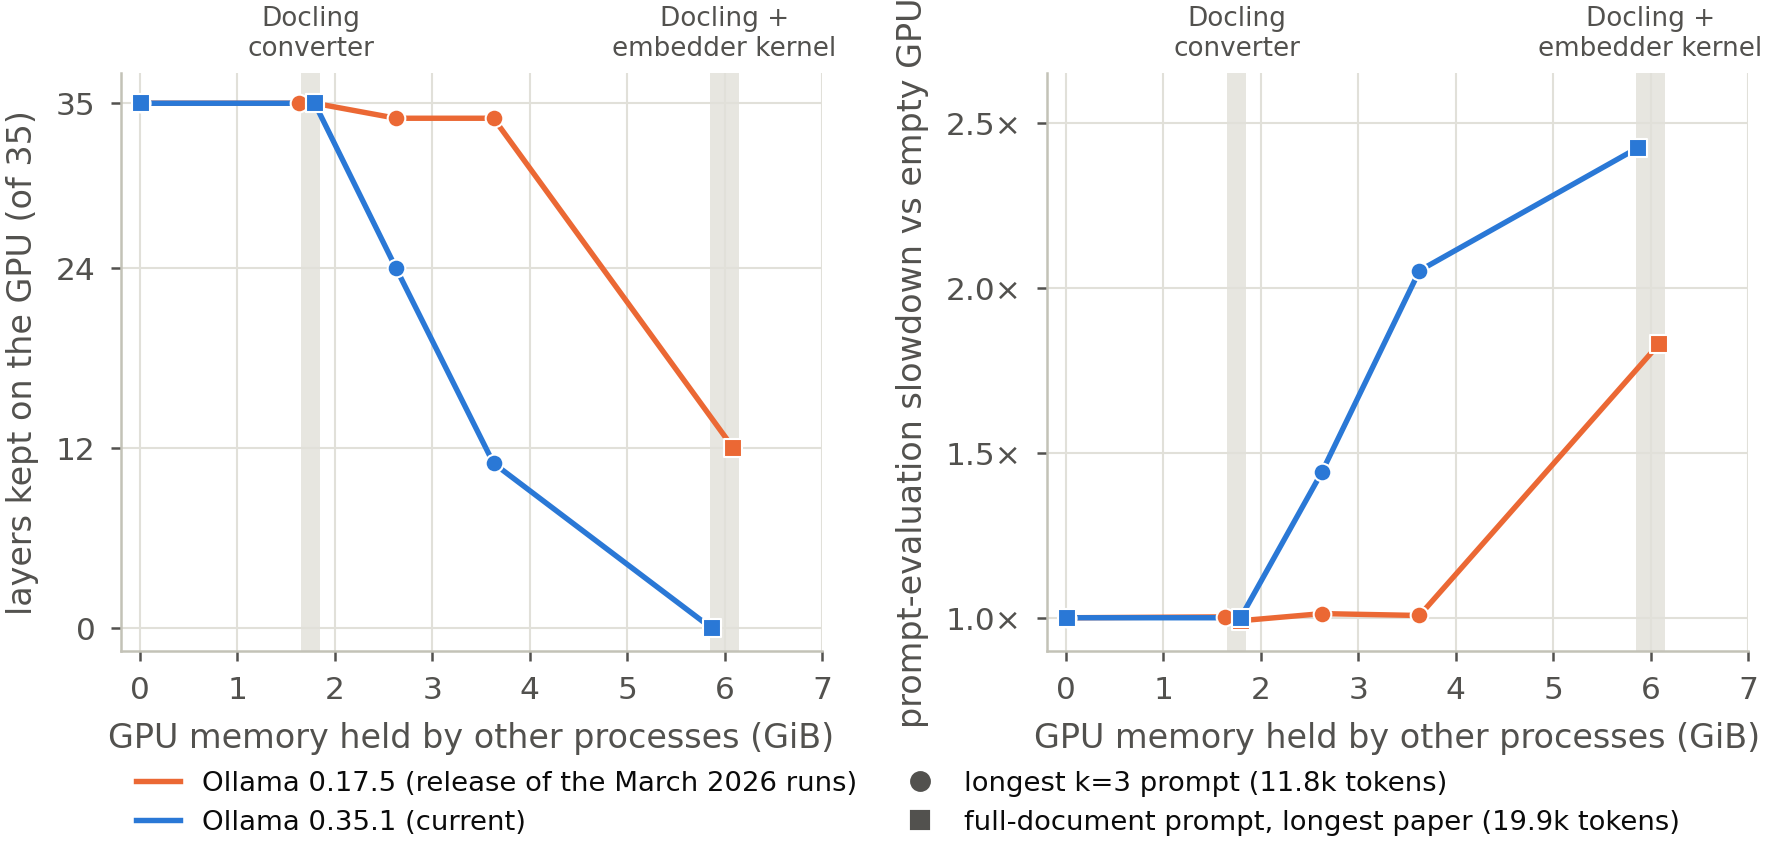
\includegraphics[width=\textwidth]{images/fig10_shared_gpu_offload.png}
  \caption{Layer placement and prompt-evaluation slowdown of the \texttt{gemma3:4b-it-qat} runner at the 30\,000-token window as a function of the device memory other processes already hold, for the server release of the March runs (0.17.5) and the current one (0.35.1); circles: longest $k=3$ prompt, squares: full-document prompt of the longest paper. Shaded bands: measured footprint of the Docling converter (1.8\,GiB) and of a kernel that has parsed and embedded the corpus (5.9--6.1\,GiB).}
  \verify{\texttt{30000} entries of \texttt{RnD/verification/ollama\_offload\_pressure\_*.json} (\texttt{gpu\_before\_load\_mib}, \texttt{offloaded\_layers}, \texttt{warm\_prompt\_eval\_s}); drawn by \texttt{RnD/citds\_article/figures/fig10\_shared\_gpu\_offload.py}}
  \label{fig:offload}
\end{figure}

\section{Discussion}\label{sec:discussion}

\subsection{Practical applicability}
For an authority indexing thousands of pages on-premises, the relevant trade-off is between accuracy and time and energy. On it the full-document baseline buys its last 0.2 points of \Rec{20} with 8.1 times the generation energy and 6.3 times the wall-clock of the routed pipeline, and the static $k=3$ slice sits in between, at half the baseline's energy for a 0.9-point loss.\verify{$106.68/13.22=8.07$ and $3294.3/525.3=6.27$ from Table~\ref{tab:primary}; $0.954-0.94533=0.0087$} Because every recall gap lies inside the $\pm0.7$-point band of a single run while the energy gaps exceed run-to-run variation by an order of magnitude, the Pareto choice is unambiguous: bounded, routed contextualisation dominates, and the savings scale with corpus size, recur at every re-index and grow with document length through the baseline's paging penalty. The router's development path (0.938, 0.942, 0.9487, 0.952) shows that its gain came from the class-to-radius mapping rather than from prompt wording; it costs one token per chunk, about a minute per corpus, and no second model. Its limits are equally clear: the oracle headroom above fixed $k=2$ is 1.7 points, and the summariser's run-to-run variation is of the same order, so further gains must come from the summariser or from multi-run evaluation.\verify{path and headroom: Sects.~1, 3 and 8 of \texttt{RnD/router\_prompt\_engineering.md}; $0.964-0.94667=0.017$}

\subsection{Limitations and future directions}
The slice is intra-document: a chunk whose meaning depends on another document, an annex cited in a report or a standard referenced by an audit, receives no help. Thousand-page audit or financial filings have not been tested; Proposition~\ref{prop:complexity} predicts the largest gains there, but also the largest exposure to cross-section dependencies. The natural extension is edge-to-cloud collaborative routing: the agent already exposes a confidence margin, so near-tie chunks, or questions a local generator cannot answer from the retrieved context, can be escalated selectively to a larger model while low-entropy work stays local. Next steps are a router run on the policy corpus with policy-specific exemplars, memory instrumentation during the benchmark runs themselves rather than after the fact (Sect.~\ref{sec:profiling}), and sufficient repeated generations to replace single-run bands with interval estimates.

\section{Conclusion}\label{sec:conclusion}

Index-time contextual retrieval can be made to fit the memory, time, and energy budget of a single consumer GPU without giving up its accuracy: bounding each chunk's context to a window of neighbors makes prompt length and reserved memory independent of document length, and a one-token routing decision of the same small model removes a third of the summaries and most of the remaining cost. On 250 multi-hop questions over 25 scientific papers the routed pipeline matched full-document contextualisation within the noise of a single run (\Rec{20} 0.952 against 0.954) with better ranking metrics, at 12\,\% of its generation energy and 16\,\% of its generation time, and the fixed-radius variant transferred to European Commission policy documents with the same accuracy gap and a 72\,\% energy saving.\verify{$13.22/106.68=0.124$ and $525.3/3294.3=0.159$ (Table~\ref{tab:primary}); $1-5.08/18.00=0.718$ (Table~\ref{tab:policy})} The pipeline is precise (its metrics are reproducible per question), explainable (every routing decision is logged with its evidence) and provable (every run carries an energy and emission ledger), the PEP-AI footing we consider necessary for AI-assisted compliance auditing at the edge of the energy system.

\backmatter

\bmhead{Acknowledgements}
An earlier version of this work was presented at the Student Research Conference of the University of Debrecen and published as a conference paper \cite{sandor2025documentslicecontextualretrieval}. It was supported by the UD Talent Program, the Doctoral School of Informatics, and the Faculty of Informatics of the University of Debrecen.

The authors acknowledge the use of generative artificial intelligence tools, namely Gemini (Google), Claude (Anthropic), ChatGPT (OpenAI), and Grammarly, in preparing this manuscript and the associated research: for language editing; Gemini for the initial literature survey and for generating the silver-standard question sets under the protocol of Section ~\ref{sec:datasets}; Gemini and ChatGPT as coding assistants; and Claude to draft and condense this journal version from the conference manuscript and the repository's experimental records, including the bibliography entries marked as machine-added in the source file, and to run the dynamic-radius routing experiments under the authors' direction. The core concepts, methodology, and scientific contributions are the authors' original work; all AI-generated outputs were produced under human supervision, validated manually, and critically reviewed and edited by the authors, who remain fully responsible for the accuracy, integrity, and originality of the content.

\section{Declarations}

\begin{itemize}
\item \textbf{Funding:} UD Talent Program; Doctoral School of Informatics and Faculty of Informatics, University of Debrecen \todo{[confirm grant identifiers, if any]}.
\item \textbf{Conflict of interest:} The authors declare no competing interests.
\item \textbf{Ethics approval and consent to participate:} Not applicable.
\item \textbf{Consent for publication:} Not applicable.
\item \textbf{Data availability:} The frozen chunk files, question sets, per-run energy records (\texttt{emissions.csv}), routing records and per-question retrieval results analysed in this article are available in the project repository \cite{sandor2025documentslicecontextualretrieval}.
\item \textbf{Materials availability:} Not applicable.
\item \textbf{Code availability:} The complete pipeline (parsing, routing agent, slice generation, indexing, evaluation and the offline policy simulator) is available in the same repository \cite{sandor2025documentslicecontextualretrieval}.
\item \textbf{Author contribution:} \todo{[insert CRediT statement]}.
\end{itemize}

\bibliography{refs}

\end{document}